\section{Basic usage}
\noindent
From this point onwards, this guide makes the following assumptions:
\begin{enumerate}
	\item 3D Slicer has been successfully installed
	\item The data you wish to work on has already been acquired
	\item The computer running 3D Slicer has access to the data
\end{enumerate}

\subsection{Loading Data}
3D Slicer can load data in two different ways.
Loading data from file or folder or load data from folder and save to database (\ref{fig:toolbar}:2).
The database option is advisable if you are dealing with a larger number of studies, as it enables quick switching between studies.
If only a single study needs to be loaded, usage of the database is not necessary.
Clicking on the \texttt{Add Data} Button (\ref{fig:toolbar}:2) or using the keyboard shortcut \texttt{Ctrl + o} brings up a file picker dialogue.
\begin{figure}[h!]
	\centerline{
		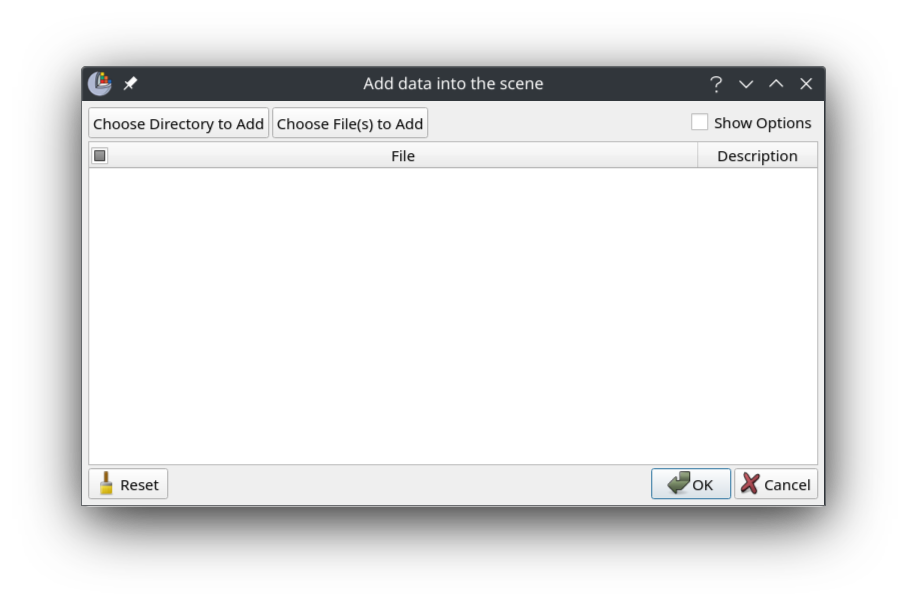
\includegraphics[
			% scale=0.2
			width=1.1\textwidth
		]{filepicker.png}}
	\caption{3D Slicer file picker}\label{fig:filepicker}
\end{figure}

\begin{figure}[h!]
	\centerline{
		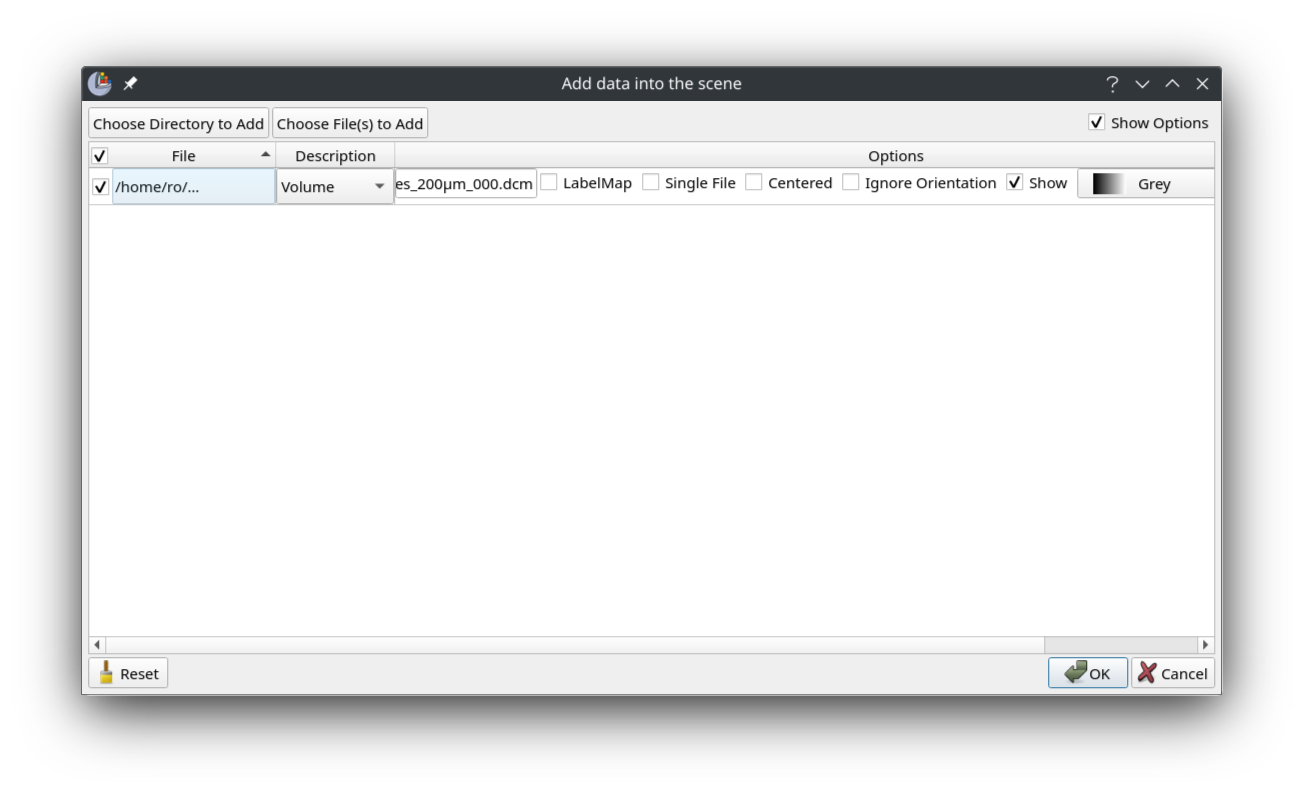
\includegraphics[
			% scale=0.2
			width=1.1\textwidth
		]{filepicker2.png}}
	\caption{3D Slicer file picker options}\label{fig:filepicker2}
\end{figure}
\noindent
Depending on whether the data is contained in a single or multiple files, click either \texttt{Choose Directory to Add} or \texttt{Choose File(s) to Add}. Browse to your data, select it and confirm your selection by clicking \texttt{Choose}.
Show additional import options by setting a checkmark at \texttt{Show Options}.
Here it is possible to load the dataset as a Label map, force 3D Slicer to ignore similar files, automatically center the volume, ignore orientation information in the DICOM header, show or hide the volume and set the color table.
After confirming the import, depending on size of the dataset, some patience may be required. If the import was successful and the dataset has not been set to be hidden after import, 3D Slicer will automatically populate the view area.

\subsection{Saving Data}
\begin{figure}[h!]
	\centerline{
		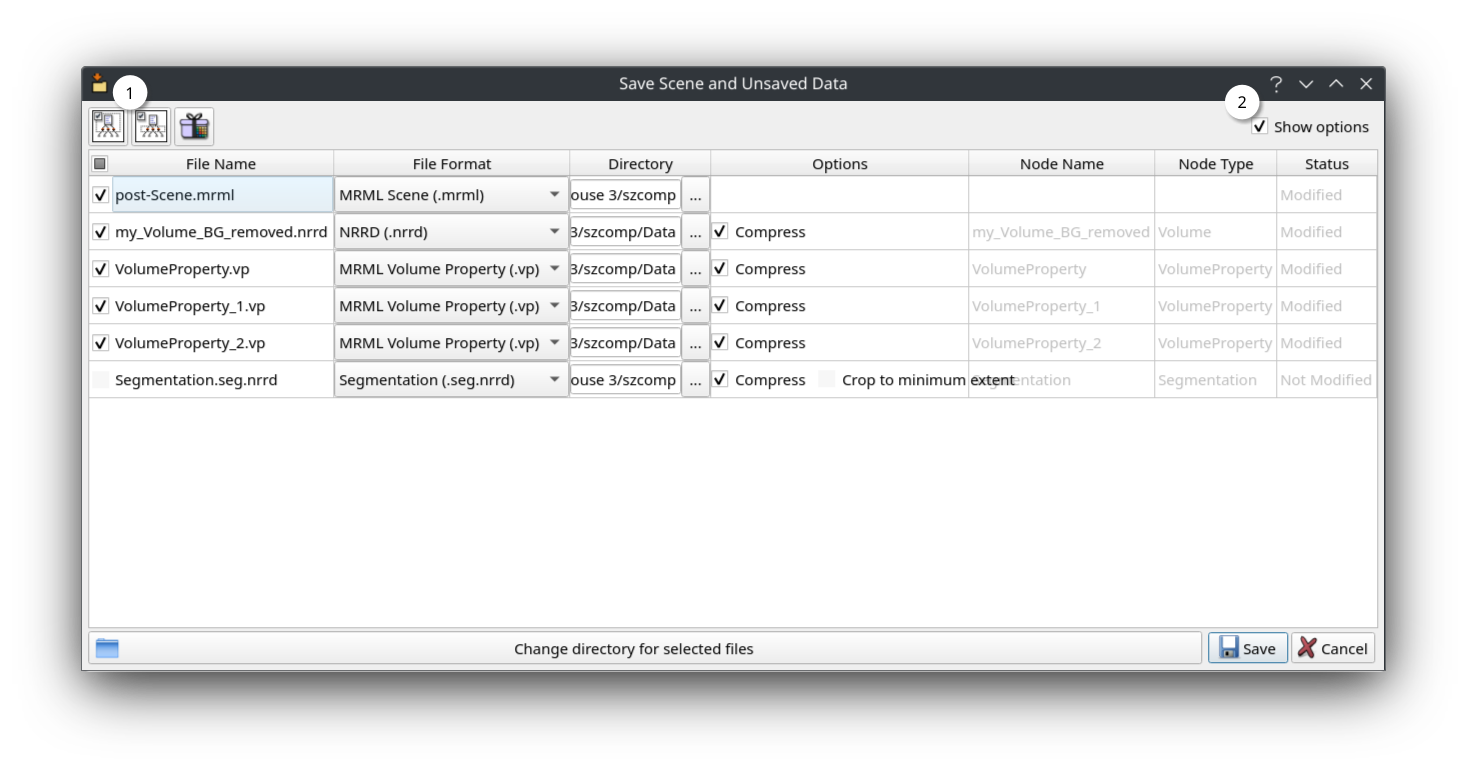
\includegraphics[
			% scale=0.2
			width=1.1\textwidth
		]{saveMenu.png}}
	\caption{3D Slicer file save menu}\label{fig:save}
\end{figure}
\noindent
Save your work in 3D Slicer by clicking on the \texttt{Save Data} button in the \cref{fig:toolbar}:3.
This will open a popup window which holds information about what data will be saved and the format it will be saved to.
3D Slicer defaults to bundling up your data into a single file. Change this by clicking on the bundle icon (\cref{fig:save}:1) and set a checkmark at \texttt{Show options} (\cref{fig:save}:2).
The window should now look like \Cref{fig:save}.
The first column shows the file names, which are derived from their names in the \texttt{Data} module and their file format.

Let us take a look at what 3D Slicer is going to save:

\begin{description}
	\item [post-Scene.mrml] \textquote{MRML file is a xml-formatted text file with scene metadata and pointers to externally stored data files}\cite{kikinis3DSlicerPlatform2014} (Metadata file)
	\item [my\_Volume\_BG\_removed.nrrd] volume data in a non-DICOM general purpose multidimensional format
	\item [VolumeProperty.vp] volume property file storing information on volume rendering (Metadata file)
	\item [Segmentation.seg.nrrd] \textquote{Segmentation labelmap representation}\cite{kikinis3DSlicerPlatform2014} storing the segmentation as a multidimensional volume
\end{description}

3D Slicer defaults to compressing all data before saving and there should be no reason to turn this behavior off.
\noindent
The second column is dedicated to the file format of the mentioned files.
3D Slicer supports a number of different file formats (see: \url{https://slicer.readthedocs.io/en/latest/user_guide/data_loading_and_saving.html#supported-data-formats}).
However, exporting for example a volume or segmentation in a different format, say STL for 3D printing, I recommend choosing the \texttt{Data} module over changing file formats in the save dialogue.
Compression can be turned off or on per file in the option's column.
And somewhat importantly, the last column, the status column, shows if a file has been modified since the last save.

Clicking on the ``Bundle'' icon (\Cref{fig:save}:1) collapses the file view, as this instructs 3D Slicer to not save individual files, but bundle them in a \Gls{mrb} file.

Pick a directory by clicking on \texttt{Change directory for selected files} and confirm via the save icon.
Depending on the file size this operation may require some patience.

\pagebreak

\subsection{Addressing Performance issues}\label{section:perf}
If loading the data took a long time or scrolling in the 2D views is sluggish, it might be worth considering reducing the size of your dataset.
Make sure to save after every operation to reduce the loss of progress in case of a crash.

\subsubsection{Cropping}\label{section:crop}
Locate the \texttt{Crop Volume} module either via the dropdown menu (\cref{fig:toolbar}) \texttt{Converters -> Crop Volume} switch to it.
\begin{figure}[h!]
	\centerline{
		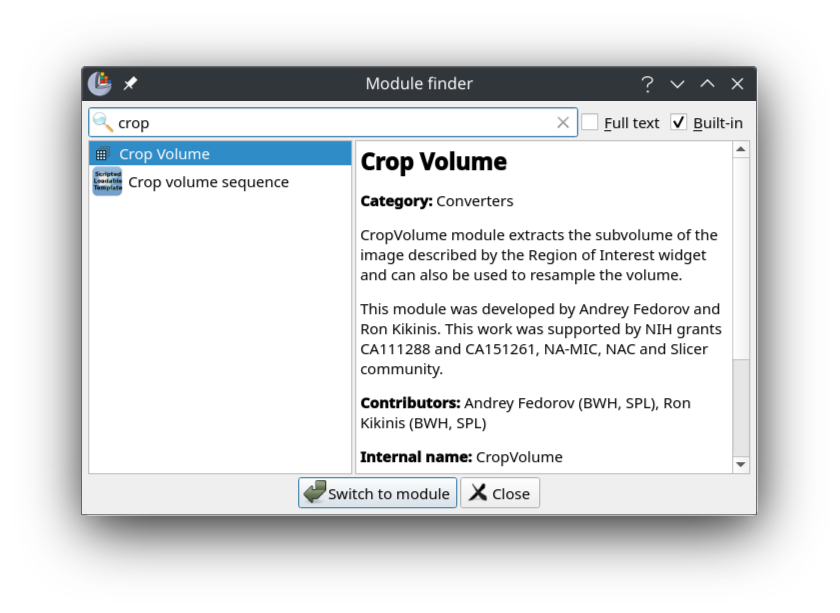
\includegraphics[
			% scale=0.2
			width=1.1\textwidth
		]{moduleSwitcher.png}}
	\caption{3D Slicer module switcher}\label{fig:mS}
\end{figure}
Or click the lens icon to use the text search (\cref{fig:mS})
Before any cropping can happen it is required to do some setup in the newly opened module panel.
\newline
\begin{figure}[h!]
	\centerline{
		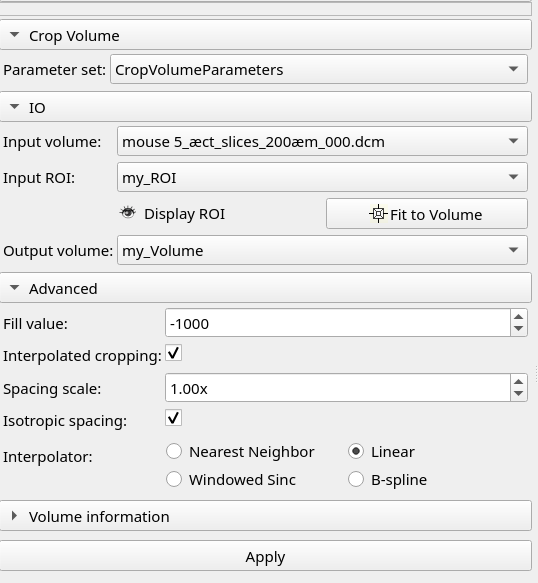
\includegraphics[
			scale=0.8
			%width=0.90\paperwidth
		]{croppingModulePanel.png}}
	\caption{3D Slicer cropping module panel}\label{fig:cMP}
\end{figure}
\newline
\noindent
See \cref{fig:cMP} for reference.
Under \texttt{IO -> Input Volume} make sure the dataset you loaded is selected.
Create a new ROI under \texttt{IO -> Input ROI} choose \texttt{Create new ROI as\ldots} and give it a distinctive name. Also make sure it is not hidden by looking for an open eye next to \texttt{Display ROI}.
\newline % sample hint
\newline % 2d, 3d, hint, irr, perf, plugin
\begin{minipage}{0.4\textwidth}
	\begin{center}
		\includesvg[
			inkscapelatex=false,
			width = 0.5\textwidth
		]{hint.svg}
	\end{center}
\end{minipage}%
%
\begin{minipage}{0.5\textwidth}
	To get a better visualization of the volume that is going to remain define the ROI in the \texttt{Volume rendering} module.
\end{minipage}
\newline
\noindent
Next choose a name for your output volume under \texttt{IO -> Output volume -> Create new volume as\ldots} and give it a distinctive name.
Under \texttt{Advanced -> Fill value} choose a HU value for everything outside your ROI. It should be easily distinguishable from the structure or tissue you are segmenting. For bone segmentation I recommend choosing -1000 HU\footnote{The HU value of air}. Checking the tick box \texttt{Advanced -> Interpolated cropping} will ensure that the output volume has the same dimensions as the input volume.
Also check the box: \texttt{Advanced -> Isotropic spacing} with a \texttt{Spacing scale} of 1x to ensure the voxels stay isotropic.
Now adjust your ROI in the 2D view areas by clicking and dragging the colored dots at the edges and corners of the ROI.
Crop out as much excess volume as possible without affecting the anatomy you wish to segment.
Check positioning and size of your ROI by scrolling through the 2D view on all three planes, after that click \texttt{Apply}.
This operation might require some patience depending on the size of the dataset.
Note that there will be no visual confirmation the cropping operation is finished.
However, you can check by switching to the \texttt{Data} module.
If 3D Slicer is unresponsive, the operation is not done yet.
\newline
\begin{figure}[h!]
	\centerline{
		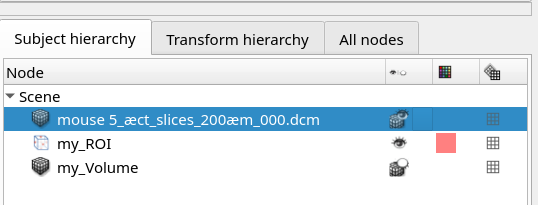
\includegraphics[
			scale=0.9
			%width=0.90\paperwidth
		]{cropConfirm.png}}
	\caption{3D Slicer data module}\label{fig:cC}
\end{figure}
\newline
\noindent
Under \texttt{Subject hierarchy -> Node -> Scene} (\cref{fig:cC}) you should see:
\begin{enumerate}
	\item the loaded dataset
	\item the newly created ROI
	\item the newly created volume
\end{enumerate}
Show your cropped volume by clicking on the closed eye on the same line as its name. Hide the ROI by clicking on the open eye next to its name.
3D slicer will then automatically hide the original dataset and populate the view area with the cropped volume dataset.

\subsubsection{Masking}\label{mask}
In the last step we cropped out the part of the source volume which does not contain any material or tissue of interest.
This step is dedicated to homogenizing the volume which was not cropped out in the last step.
\begin{figure}[h!]
	\centerline{
		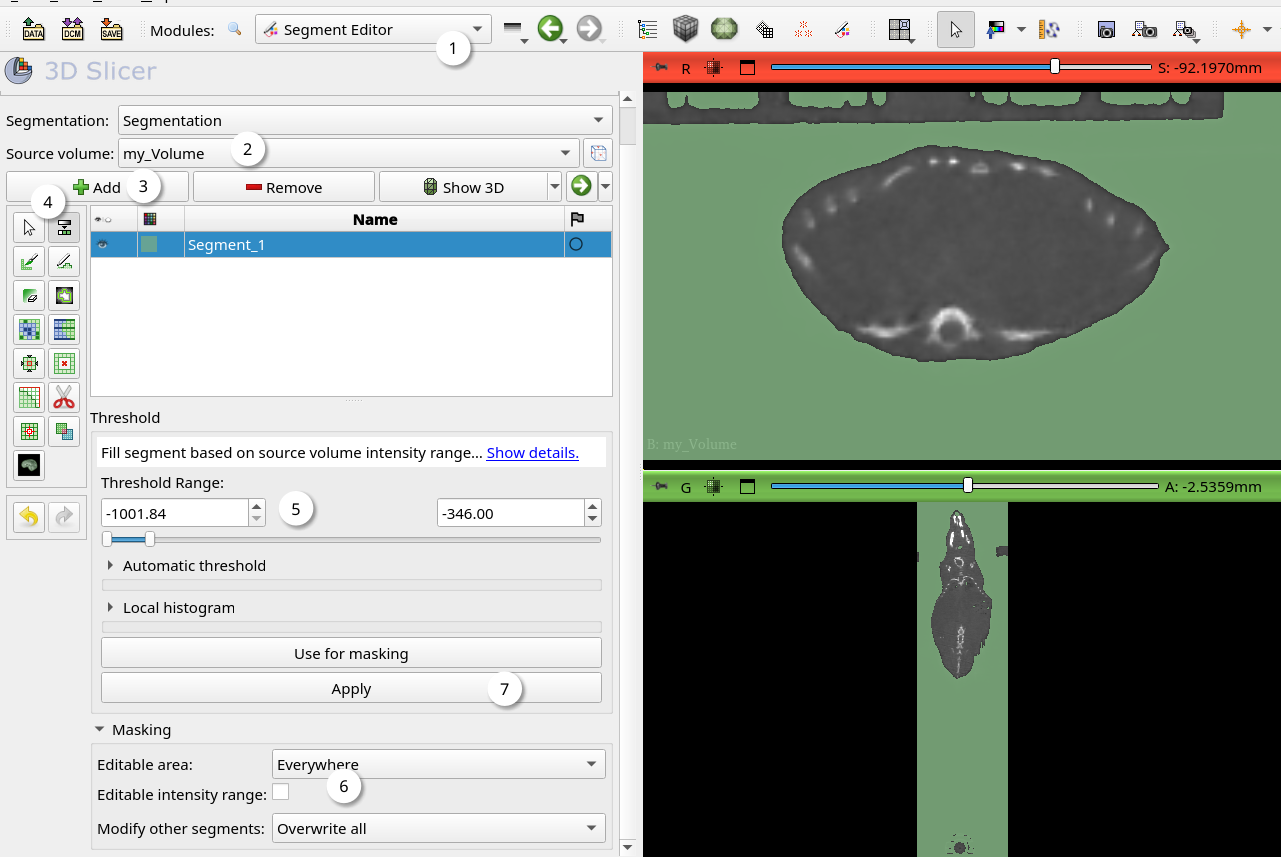
\includegraphics[
			%scale=0.5
			width=1.1\textwidth
		]{thesholdMasking.png}}
	\caption{Threshold background}\label{fig:tM}
\end{figure}
Switch to the \texttt{Segment Editor} module (\cref{fig:tM}:1).
Make sure your cropped volume is selected as the \texttt{Source volume} (\cref{fig:tM}:2).
Click on the \texttt{+ Add} button (\cref{fig:tM}:3). You should see a new segment appear in the segments list below.
Double click to rename it to ``Background'' or leave its default name.
Make sure your ``Background''segment is select and then activate the \texttt{Threshold} tool (\cref{fig:tM}:4).
Shift the lower threshold limit until the background is covered by the segment color in the 2D views. Afterward shift the upper threshold limit until your tissue of interest is definitely no longer covered by the segment color.
Before applying (\cref{fig:tM}:7) the threshold segmentation make sure that 3D Slicer is allowed to edit \texttt{Everywhere} and overwrite all other segments (\cref{fig:tM}:6).

\pagebreak
\begin{figure}[h!]
	\centerline{
		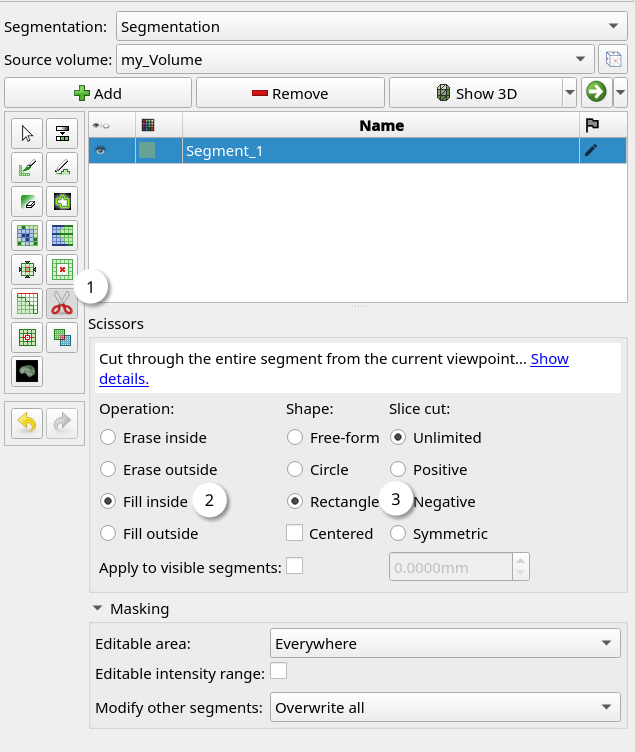
\includegraphics[
			scale=0.8
			%width=0.80\paperwidth
		]{scissorsMasking.png}}
	\caption{Scissors background}\label{fig:sM}
\end{figure}
\noindent
Next, activate the \texttt{Scissors} tool (\cref{fig:sM}:1) with your ``Background'' segment selected.
This tool provides a simple way of selecting materials and tissue that are not easily distinguished by HU value, like the MicroCT couch and positioning tools.
Change its operation mode to \texttt{Fill inside} (\cref{fig:sM}:2) and its shape to \texttt{Rectangle} or \texttt{Free-form} (\cref{fig:sM}:3).
In the 2D views you can now click and drag to create a shape, upon releasing the left mouse button, the tool will add the volume inside the shape to your ``Background'' segment.
\newline % sample hint
\newline % 2d, 3d, hint, irr, perf, plugin
\begin{minipage}{0.4\textwidth}
	\begin{center}
		\includesvg[
			inkscapelatex=false,
			width = 0.5\textwidth
		]{hint.svg}
	\end{center}
\end{minipage}%
%
\begin{minipage}{0.5\textwidth}
	The scissors tool ``punches'' through the volume, this makes it very easy to accidentally select something intentionally.
	Always make sure there is no ROI in the area on the previous or next slices and check your positioning on the other planes.
	In most cases it will be easier to work on small sections of your volume, rather than selecting a large volume in one single step.
\end{minipage}

\pagebreak
\begin{figure}[h!]
	\centerline{
		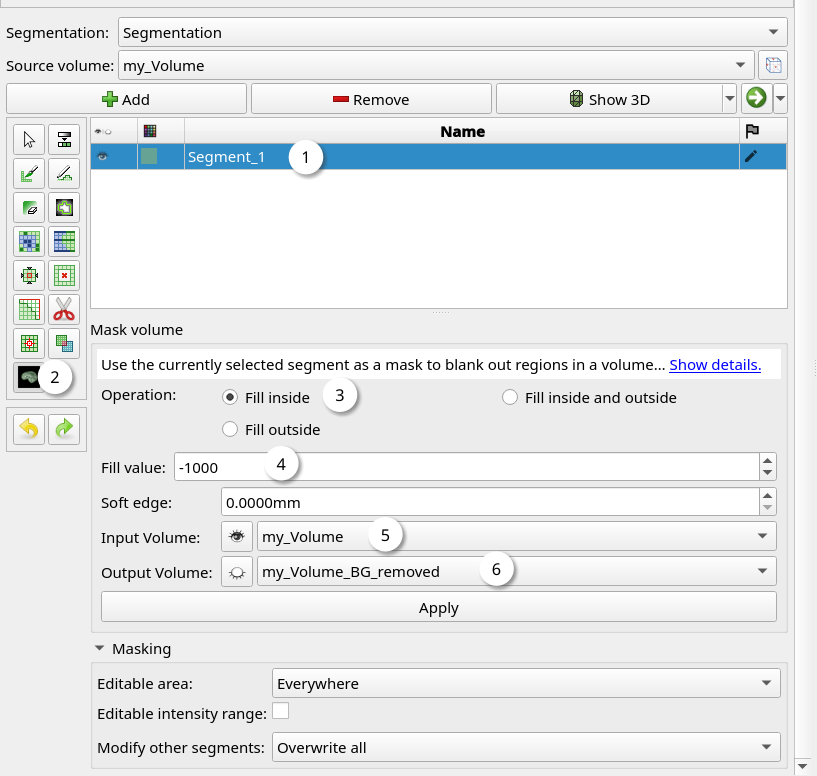
\includegraphics[
			%scale=0.8
			width=1.2\textwidth
		]{maskBG.png}}
	\caption{Mask background}\label{fig:mBG}
\end{figure}
\noindent
Activate the \texttt{Mask volume} tool (\cref{fig:mBG}:2) and make sure your ``Background'' segment is selected (\cref{fig:mBG}:1).
As for the operation mode, choose \texttt{Fill inside} (\cref{fig:mBG}:3).
The fill value (\cref{fig:mBG}:4) should be the same as in the cropping step (\cref{section:crop}).
Select your cropped source volume as the \texttt{Input Volume} (\cref{fig:mBG}:5).
For the result, create a new volume by clicking on \texttt{Output Volume -> Create new Volume as\ldots} (\cref{fig:mBG}:6) and give it a distinctive name.
\newline % sample hint
\newline
\begin{minipage}{0.4\textwidth}
	\begin{center}
		\includesvg[
			inkscapelatex=false,
			width = 0.5\textwidth
		]{irreversible.svg}
	\end{center}
\end{minipage}%
%
\begin{minipage}{0.5\textwidth}
	Always create a new volume when working with the \texttt{Mask volume} tool.
	It overrides the individual voxel intensity values, this \emph{can not be undone} as 3D Slicer does not store the original intensity values in its undo history.
\end{minipage}
\pagebreak

\subsubsection{Cleanup}
Switch to the \texttt{Data} module.
\begin{figure}[h!]
	\centerline{
		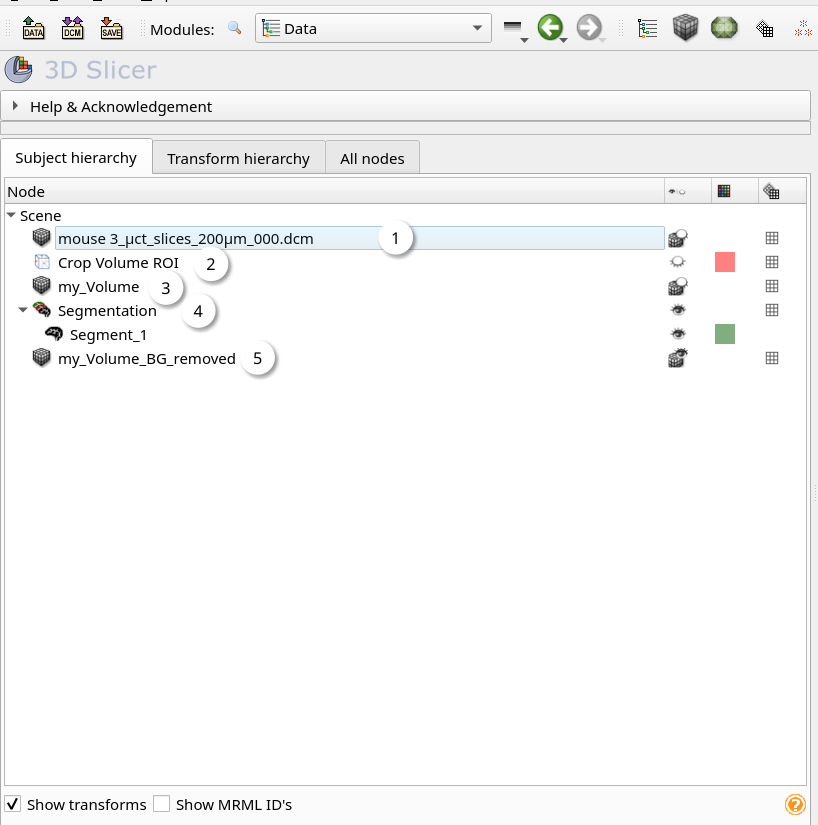
\includegraphics[
			%scale=0.8
			width=1.2\textwidth
		]{cleanup.png}}
	\caption{Data cleanup}\label{fig:clr}
\end{figure}
\noindent
Here we see all the items we have created so far.
\Cref{fig:clr}:1 is the DICOM dataset from the MicroCT scanner.
\Cref{fig:clr}:2 is the cropping ROI created in \cref{section:crop} and \cref{fig:clr}:3 is the volume that resulted from the cropping operation.
The segmentation item (\cref{fig:clr}:4) holds all segmentations created in the \texttt{Segment Editor} module. So far it only holds the ``Background'' segment created in \Cref{mask}. And the final item (\cref{fig:clr}:5) is the most recent volume resulting from the \texttt{Mask volume} operation.
Items \cref{fig:clr}:1-4 can be deleted to save harddrive space and RAM while working in 3D Slicer.
\noindent
In this example the data volume on disk could be decreased from 309 megabytes to (source DICOM data) to 15 megabytes.
Which equates to approximately a 95\% reduction in file size.
As a result of this, 3D Slicers RAM consumption has dropped from 1.3 gigabytes to 585 megabytes, which equates to approximately 55\% reduction.
See \Cref{measuements:memComp} for more information.
\newline
\begin{figure}
	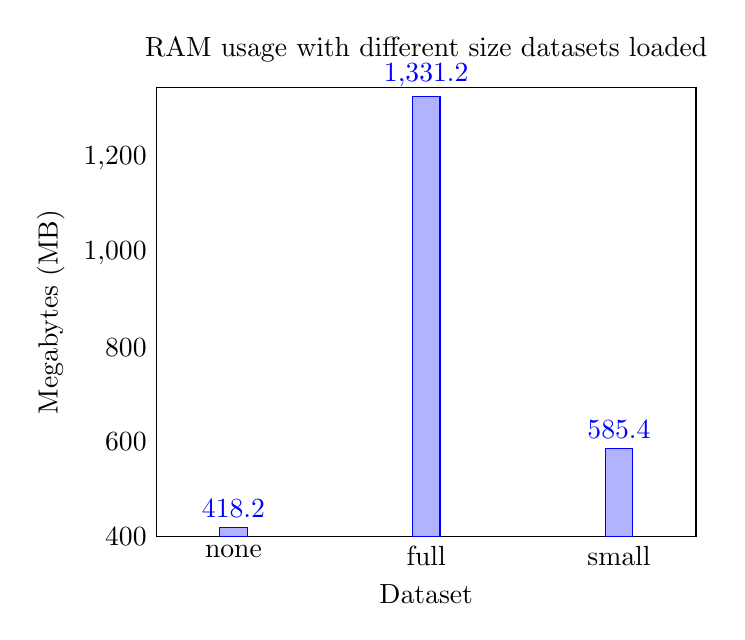
\begin{tikzpicture}
		\begin{axis}[
				title = RAM usage with different size datasets loaded,
				ybar,
				tickwidth = 0pt,
				xtick = data,
				enlarge y limits = 0.02,
				enlarge x limits = 0.2,
				ylabel={Megabytes (MB)},
				xlabel={Dataset},
				symbolic x coords = {none, full, small},
				nodes near coords
			]
			\addplot+ coordinates {
					(none, 418.2)
					(full, 1331.2)
					(small, 585.4)};
		\end{axis}
	\end{tikzpicture}
	\caption{RAM usage comparison}\label{fig:ramUC}
\end{figure}
\newline
\noindent
\Cref{fig:ramUC} is a RAM usage comparison of 3D Slicer under different workloads, with the intention of showing the user what amount of resource consumption to expect.\\
\texttt{none} refers to 3D Slicers base RAM usage without any dataset loaded.\\
\texttt{full} refers to the RAM usage with a raw dataset of 309 megabytes file size.\\
\texttt{small} refers to the RAM usage with the same dataset as above but reduced down to 15 megabytes file size using the method explained in \cref{section:perf}.
\pagebreak


\section{Segmentation tools}
With your dataset loaded and prepared switch to the \texttt{Segmentation Editor} module.
Before you start to segment \emph{ALWAYS} make sure the masking options are set correctly.
\begin{description}
	\item [Editable area] which areas are affected by your tool
	      \begin{description}
		      \item [Everywhere] no restrictions, tool is usable anywhere in the view areas
		      \item [Inside all segments] tool can overwrite any existing segment, does not work outside of segments
		      \item [Inside all visible segments] tool can overwrite any existing segment that is not hidden, does not work outside of segments
		      \item [Outside all segments] inverse of \texttt{Inside all segments}, tool works only outside existing segments
		      \item [Outside all visible segments] inverse of \texttt{Inside all visible segments}, tool works only outside existing non-hidden segments
		      \item [Inside \texttt{user created segments}] tool can override only selected existing segment, does not work outside of segment
	      \end{description}
	\item [Editable intensity range] restrict tool to affect only specific HU value range
	\item [Modify other segments] define interaction with other existing segments
	      \begin{description}
		      \item [Overwrite all] tool can overwrite all existing segments
		      \item [Overwrite visible] tool can overwrite all existing non-hidden segments
		      \item [Allow overlap] tool does not overwrite existing segments, instead segmented areas are shared between the affected segments
	      \end{description}
\end{description}
\pagebreak

\subsection{Built in segmentation tools}
\begin{figure}[h!]
	\begin{minipage}{0.6\textwidth}
		\begin{center}
			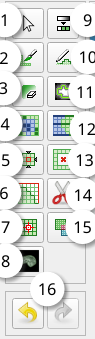
\includegraphics[
				scale=1.2
			]{segmentationTools.png}
			\caption{Segmentation tool}\label{fig:sT}
		\end{center}
	\end{minipage}%
	%
	\begin{minipage}{0.6\textwidth}
		\begin{enumerate}
			\item \texttt{No editing}
			\item \texttt{Paint}
			\item \texttt{Erase}
			\item \texttt{Grow from seeds}
			\item \texttt{Margin}
			\item \texttt{Smoothing}
			\item \texttt{Islands}
			\item \texttt{Mask volume}
			\item \texttt{Threshold}
			\item \texttt{Draw}
			\item \texttt{Level tracing}
			\item \texttt{Fill between slices}
			\item \texttt{Hollow}
			\item \texttt{Scissors}
			\item \texttt{Logical operators}
			\item \texttt{Undo and Redo}
		\end{enumerate}
	\end{minipage}
\end{figure}

\subsubsection{No editing}
Selected by default. Enables inspection of 2D and 3D views without accidentally modifying a segmentation.
\pagebreak
\subsubsection{Paint}\label{section:paint}
\begin{figure}[h]
	\begin{subfigure}{0.2\textwidth}
		\includesvg[
			inkscapelatex=false,
			width = 0.3\textwidth
		]{2d.svg}
	\end{subfigure}
	\begin{subfigure}{0.2\textwidth}
		\includesvg[
			inkscapelatex=false,
			width = 0.3\textwidth
		]{3d.svg}
	\end{subfigure}
\end{figure}
\begin{figure}[h!]
	\centerline{
		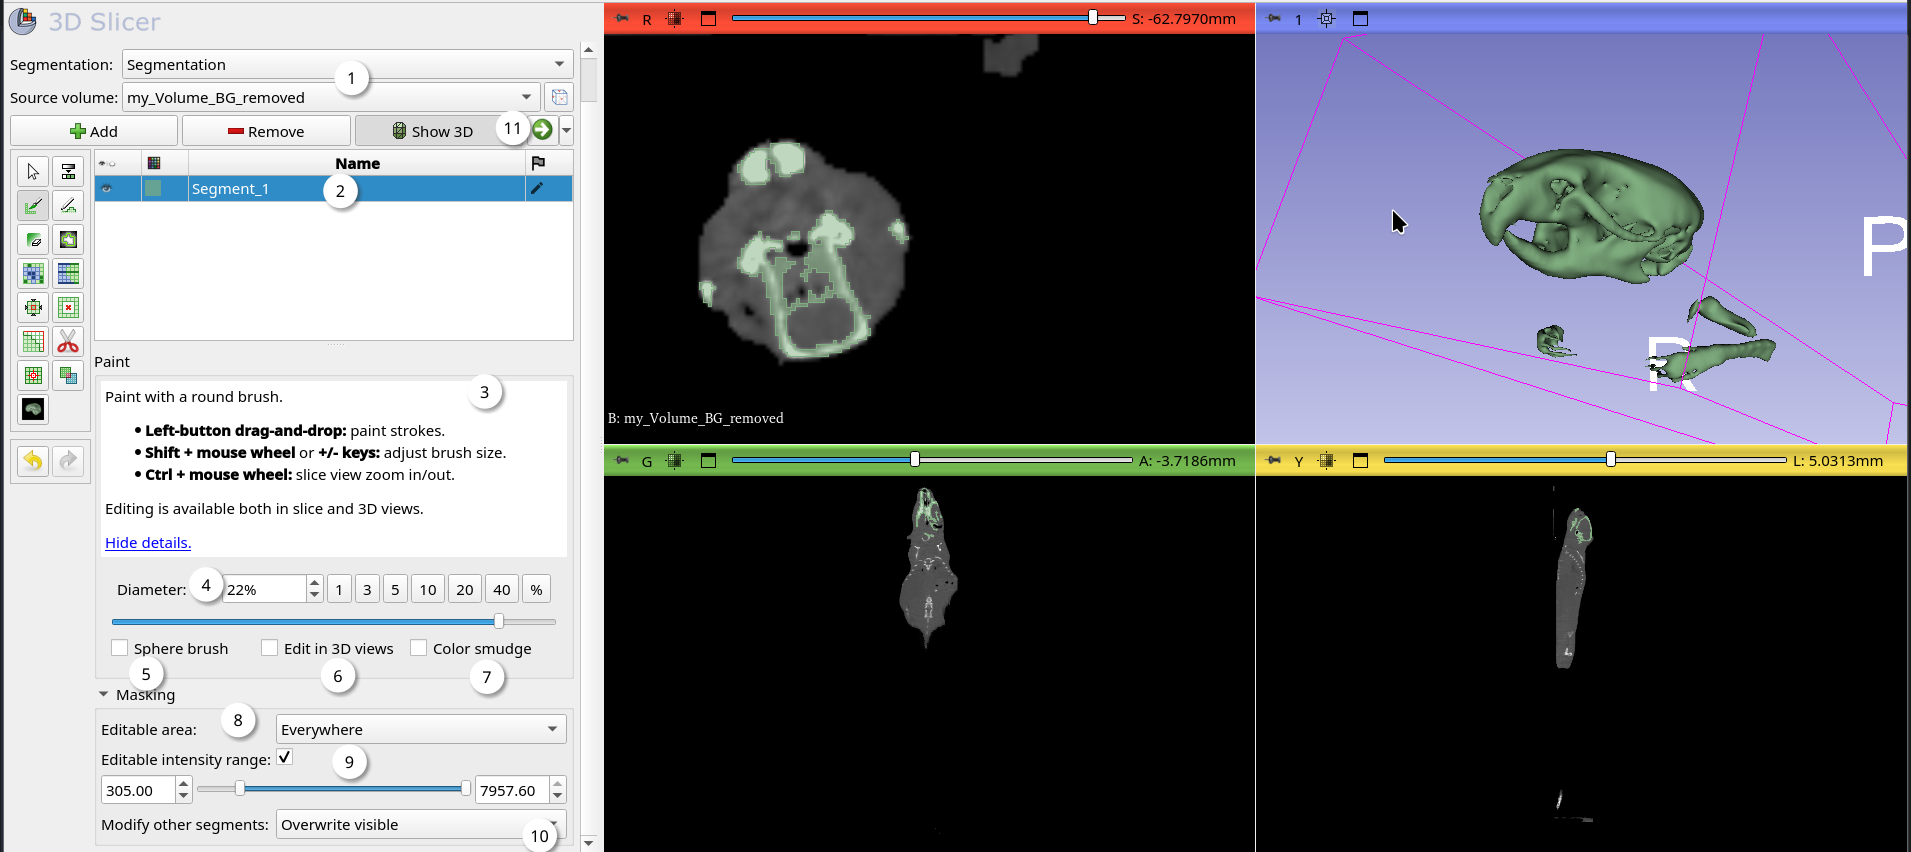
\includegraphics[
			% scale=0.2
			width=1.1\textwidth
		]{paint.png}}
	\caption{Paint tool}\label{fig:paint}
\end{figure}

\noindent
The \texttt{Paint} tool is the most widely applicable manual segmentation tool. It is also the basis for most semi-automatic segmentation tools.
To get started, first make sure the correct volume dataset and segmentation dataset are loaded (\cref{fig:paint}:1).
Create a new segment to segment a new object or organ.
Or select an existing segment to continue working on it.
Navigate to the region you wish to work on in the 2D view areas and activate the \texttt{Paint} tool.
Check your masking options before making any modifications (\cref{fig:paint}:10).
3D Slicer displays the most important keyboard options in the help area (\cref{fig:paint}:4).
Left-click and drag to draw, Shift+Mouse wheel to change the brush size, Ctrl+mouse wheel to zoom, middle mouse drag and move to pan.
\Cref{fig:paint}:4 displays the brush size modification options, click and drag the slider to increase the brush size, alternatively click one of the size presets.
In most cases setting the brush size via this menu will be not necessary, instead use the keyboard shortcuts.
Keeping the mouse in the view area during segmentation enforces a non-disruptive workflow.
Make the \texttt{Paint} tool affect more than one slice by making the brush spherical (\cref{fig:paint}:5).
The sphere brush can also be used in the 3D view if enabled (\cref{fig:paint}:6).
If you wish to allow overlapping segments, enable \texttt{Color smudge} (\cref{fig:paint}:7).

\pagebreak
\subsubsection{Erase}
Erase segmentation with brush. Inverse of Paint tool, for usage see \cref{section:paint}.

\subsubsection{Grow from seeds}\label{section:gfs}
\begin{figure}[h]
	\begin{subfigure}{0.2\textwidth}
		\includesvg[
			inkscapelatex=false,
			width = 0.3\textwidth
		]{2d.svg}
	\end{subfigure}
	\begin{subfigure}{0.2\textwidth}
		\includesvg[
			inkscapelatex=false,
			width = 0.3\textwidth
		]{performance.svg}
	\end{subfigure}
\end{figure}

\begin{figure}[h!]
	\centerline{
		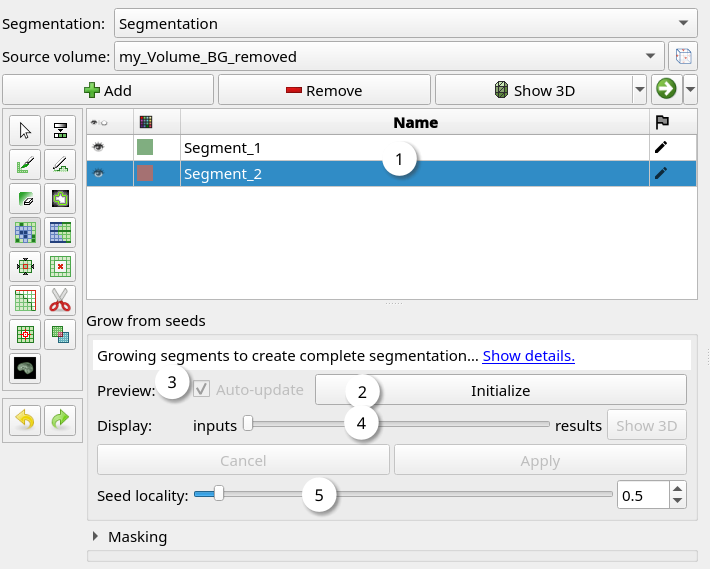
\includegraphics[
			% scale=0.2
			width=1.1\textwidth
		]{growFromSeeds.png}}
	\caption{Grow from seeds tool}\label{fig:gfs}
\end{figure}
\noindent
Semi-automatic segmentation tool based on seeds and distinctive HU changes.
To get started create at least two segments (\cref{fig:gfs}:1), one for the ``Background'' and one for the actual segmentation.
Use the paint tool to create seeds in those segments.
Try to evenly distribute seeds throughout your segmentation area in all three planes.
Additionally, try to define the border between your segments manually.
Click \texttt{Initialize} and wait for the 2D views to display the segmentation preview.
Change the opacity of the preview via the slider (\cref{fig:gfs}:4) or display it in the 3D view.
The first iteration will most likely be not satisfactory.
Turn of \texttt{Auto-update} (\cref{fig:gfs}:3) and switch back to the \texttt{Paint} tool.
Add seeds in all areas \texttt{Grow from seeds} segmented incorrectly.
Switch back to \texttt{Grow from seeds} and click \texttt{update}.
If the segmentation does not grow enough or grows disproportionate, change the seed location modifier (\cref{fig:gfs}:5).
Increasing the modifier forces the segmentation to be more localized and vice versa.
Repeat this cycle of adding seeds and letting the segmentation update until the segmentation is satisfactory.
Click apply to confirm the segmentation, delete the ``Background'' segment if its no longer useful.

%\pagebreak

\subsubsection{Margin}\label{section:margin}
\begin{figure}[h]
	\begin{subfigure}{0.2\textwidth}
		\includesvg[
			inkscapelatex=false,
			width = 0.3\textwidth
		]{2d.svg}
	\end{subfigure}
\end{figure}


\begin{figure}[h!]
	\centerline{
		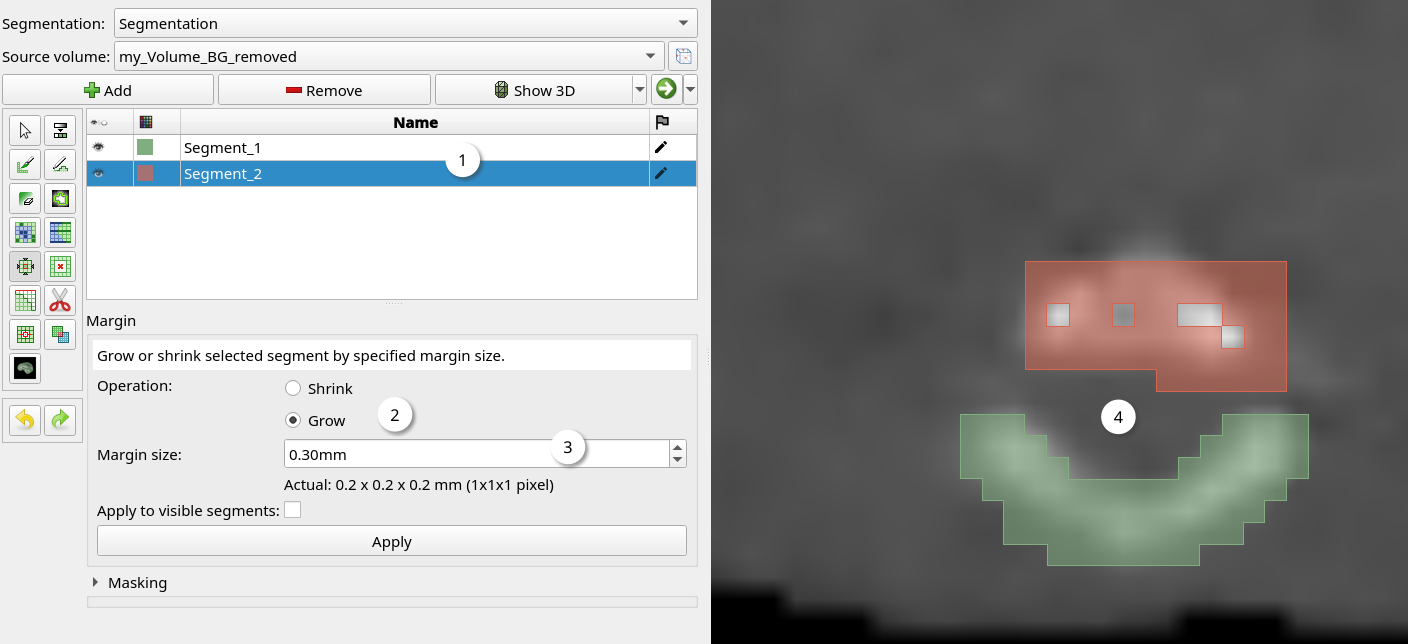
\includegraphics[
			% scale=0.2
			width=1.1\textwidth
		]{margin.png}}
	\caption{Margin tool}\label{fig:margin}
\end{figure}
\noindent
Grow or shrink a segmentation by specific amount.
Select the segment you wish to modify (\cref{fig:margin}:1).
Pick \texttt{Grow} or \texttt{Shrink} depending on your needs.
Set the size to grow or shrink by (\cref{fig:margin}:3) and click \texttt{Apply} to confirm the operation.
\newline % sample hint
\newline % 2d, 3d, hint, irr, perf, plugin
\begin{minipage}{0.4\textwidth}
	\begin{center}
		\includesvg[
			inkscapelatex=false,
			width = 0.5\textwidth
		]{hint.svg}
	\end{center}
\end{minipage}%
%
\begin{minipage}{0.5\textwidth}
	This tool can be used to fill small holes by first growing a segment slightly and then immediately shrinking it by the same amount.
	Or it can be used to separate two segments which have some overlap by shrinking both.
\end{minipage}
\pagebreak

\subsubsection{Smoothing}
\begin{figure}[h]
	\begin{subfigure}{0.2\textwidth}
		\includesvg[
			inkscapelatex=false,
			width = 0.3\textwidth
		]{2d.svg}
	\end{subfigure}
\end{figure}


\begin{figure}[h!]
	\centerline{
		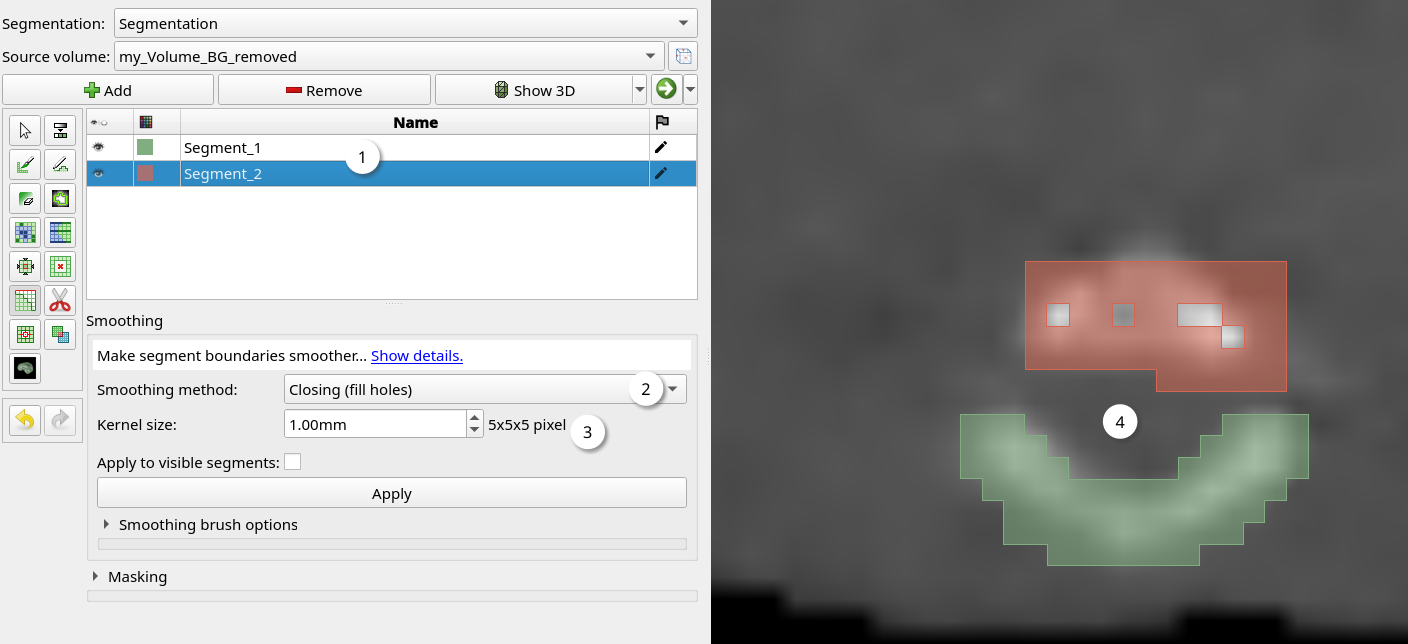
\includegraphics[
			% scale=0.2
			width=1.1\textwidth
		]{smoothing.png}}
	\caption{Smoothing tool}\label{fig:smoothing}
\end{figure}
\noindent
Smooth segmentation or fill small holes.
Select the segment you wish to modify (\cref{fig:smoothing}:1).
Select a smoothing method (\cref{fig:smoothing}:2) and kernel size (\cref{fig:smoothing}:3). If you are not sure which kernel size is best for your dataset, set the kernel size as small as possible in order to avoid large modifications.
Undo if the result is not satisfactory, increase the kernel by a small amount and try again.
\begin{description}
	\item [Median] removes small extrusion while leaving smooth areas mostly unchanged
	\item [Opening] removes extrusions smaller than the kernel size
	\item [Closing] fills holes and sharp corners smaller than the kernel size
	\item [Gaussian] smooths all contours and shrinks the segment
	\item [Joint smoothing] affects all visible segments, smooths multiple segments at once
\end{description}

\pagebreak
\subsubsection{Islands}
\begin{figure}[h]
	\begin{subfigure}{0.2\textwidth}
		\includesvg[
			inkscapelatex=false,
			width = 0.3\textwidth
		]{2d.svg}
	\end{subfigure}
	\begin{subfigure}{0.2\textwidth}
		\includesvg[
			inkscapelatex=false,
			width = 0.3\textwidth
		]{3d.svg}
	\end{subfigure}
\end{figure}


\begin{figure}[h!]
	\centerline{
		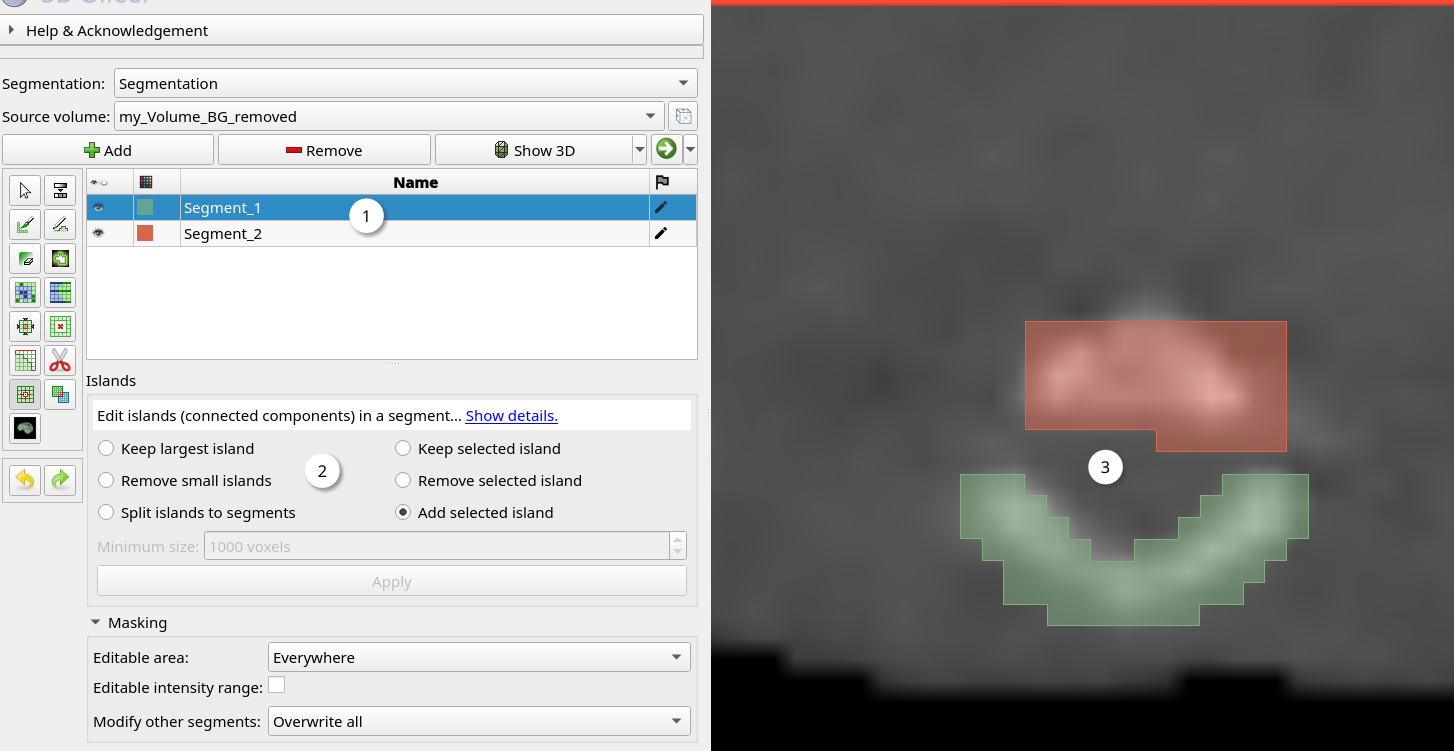
\includegraphics[
			% scale=0.2
			width=1.1\textwidth
		]{islands.png}}
	\caption{Islands tool}\label{fig:islands}
\end{figure}
\noindent
Multitool operating on disconnected segmentation areas or connected segmentation areas with different labels.
\begin{description}
	\item [Keep largest island] deletes all islands but the largest one
	\item [Remove small islands] deletes all islands smaller than the specified minimum size
	\item [Split islands to segments] deletes all islands smaller than the specified minimum size, the remaining islands will be automatically assigned a new segment each
	\item [Keep selected island] click on an island you wish to keep, all other islands will be deleted
	\item [Remove selected island] click on an island you wish to delete, all other islands will be unaffected
	\item [Add selected island] click on an island you wish to join with the selected segment, it will inherit the label of the segment
\end{description}
\pagebreak

\subsubsection{Mask volume}\label{section:mask}
\begin{figure}[h]
	\begin{subfigure}{0.2\textwidth}
		\includesvg[
			inkscapelatex=false,
			width = 0.3\textwidth
		]{2d.svg}
	\end{subfigure}
	\begin{subfigure}{0.2\textwidth}
		\includesvg[
			inkscapelatex=false,
			width = 0.3\textwidth
		]{irreversible.svg}
	\end{subfigure}
\end{figure}


\begin{figure}[h!]
	\centerline{
		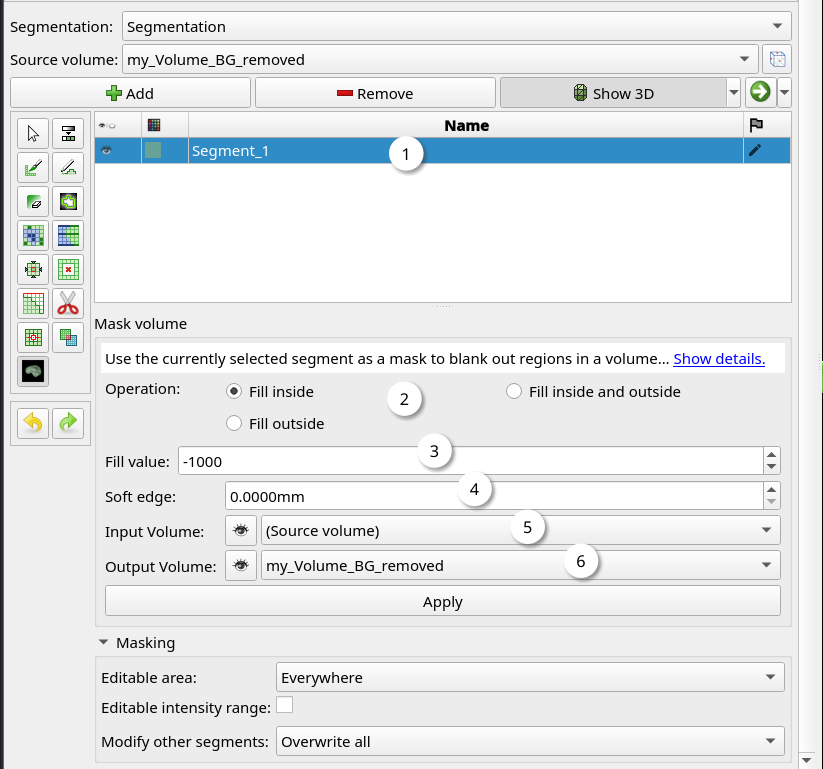
\includegraphics[
			% scale=0.2
			width=1.1\textwidth
		]{maskVolume.png}}
	\caption{Mask volume tool}\label{fig:mv}
\end{figure}

\noindent
Tool to overwrite parts of a volume.
\newline % sample hint
\newline % 2d, 3d, hint, irr, perf, plugin
\begin{minipage}{0.4\textwidth}
	\begin{center}
		\includesvg[
			inkscapelatex=false,
			width = 0.5\textwidth
		]{irreversible.svg}
	\end{center}
\end{minipage}%
%
\begin{minipage}{0.5\textwidth}
	\texttt{Mask volume} overwrites HU values in your dataset and 3D Slicer does not save the previous values in its undo history.
	Thus, if you accidentally overwrite something unintentionally you will not be able to undo your action.
	When using this tool \emph{always} save your progress and make a backup copy of your save file.
\end{minipage}

To get started, create and select a segment you wish to modify (\cref{fig:mv}:1).
The segment can for example be the background you wish to blank out.
Or it can be an object or organ you wish to blank out or preserve.
In the example \Cref{fig:mv} \texttt{Mask volume} was used to blank out the background, some support structures and just preserve the scanned animal.
This was achieved by using the \texttt{Threshold} tool (\cref{section:threshold}) to segment the air.
Then the \texttt{Scissors} tool (\cref{section:scissors}) was used to segment the positioning and support structures.
Next, select an operation mode (\cref{fig:mv}:2) and fill value (\cref{fig:mv}:3).
\newline
\begin{description}
	\item [Fill inside] fill volume inside selected segment with \texttt{Fill value}
	\item [Fill outside] fill volume outside selected segment with \texttt{Fill value}
	\item [Fill inside and outside] takes two fill values (inside and outside), fill volume inside and outside with these values respectively
\end{description}
The tool can also smooth the edge between segments with a blur. Increase the \texttt{Soft edge} (\cref{fig:mv}:4) value above zero.
Before applying the operation, make sure the correct \texttt{Input Volume} is selected and create an \texttt{Output Volume}.

%\pagebreak

\subsubsection{Threshold}\label{section:threshold}
\begin{figure}[h]
	\begin{subfigure}{0.2\textwidth}
		\includesvg[
			inkscapelatex=false,
			width = 0.3\textwidth
		]{2d.svg}
	\end{subfigure}
\end{figure}


\begin{figure}[h!]
	\centerline{
		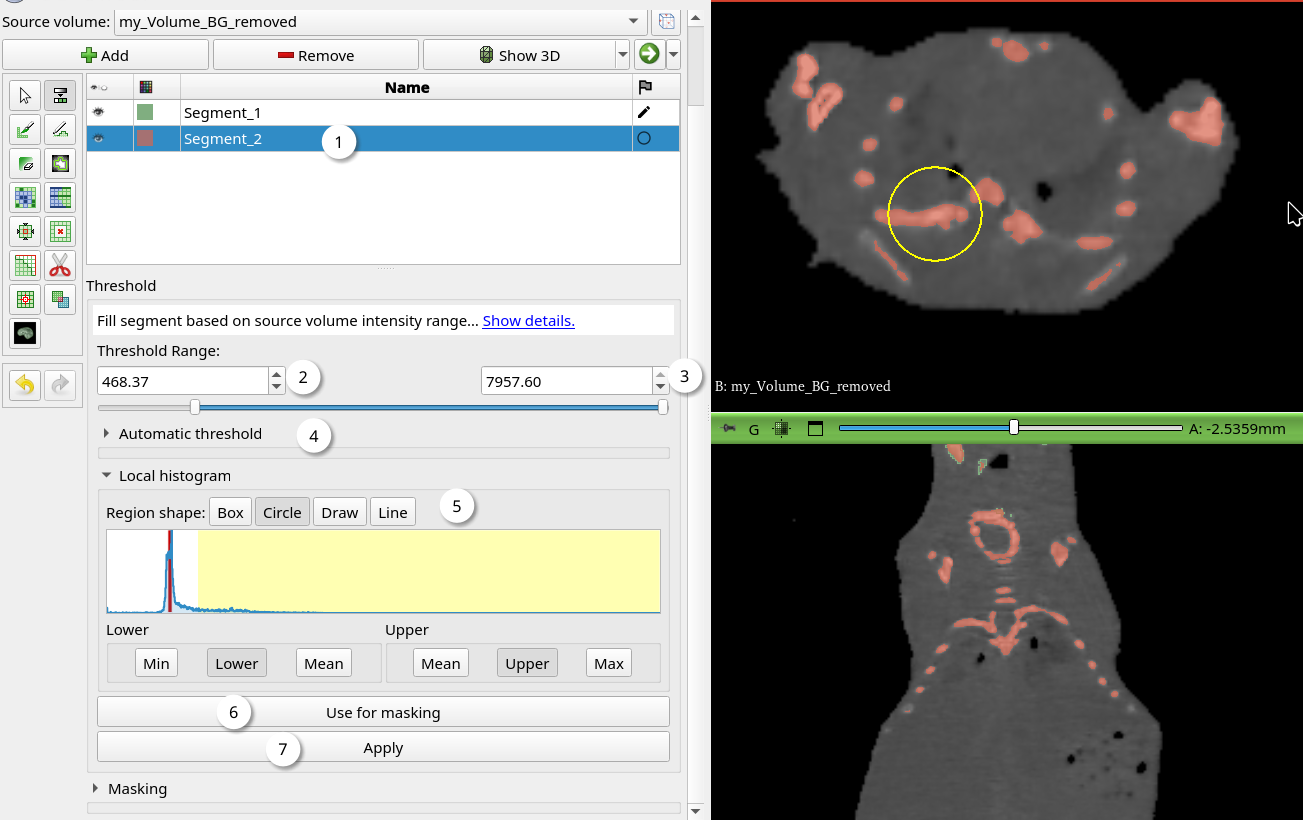
\includegraphics[
			% scale=0.2
			width=1.1\textwidth
		]{threshold.png}}
	\caption{Threshold tool}\label{fig:threshold}
\end{figure}
\noindent
Segment by HU value range.\\
First, select the segment to threshold (\cref{fig:threshold}:1).
Next, pick a lower (\cref{fig:threshold}:2) and upper (\cref{fig:threshold}:3) limit either by clicking and dragging the sliders or by typing in the HU values manually.
A dynamically updated preview will be available in the 2D views.
Automatic threshold algorithms (\cref{fig:threshold}:4) can be used to determine the limits but in most cases clicking and dragging the slider will be faster.
You may want to see a histogram of a ROI and pick your lower and upper limit from the histogram (\cref{fig:threshold}:5).
In order to do that, pick a ROI shape and click and drag it in a 2D view area.
Click on the histogram to choose your limits.
If you do not want to save your threshold to a segment but intend to use it for masking with the \texttt{Paint} tool, click on \texttt{Use for masking} (\cref{fig:threshold}:6).
This will activate the \texttt{Paint} tool with your threshold limits set as the masking option.

\pagebreak
\subsubsection{Draw}\label{section:draw}
\begin{figure}[h]
	\begin{subfigure}{0.2\textwidth}
		\includesvg[
			inkscapelatex=false,
			width = 0.3\textwidth
		]{2d.svg}
	\end{subfigure}
\end{figure}


\begin{figure}[h!]
	\centerline{
		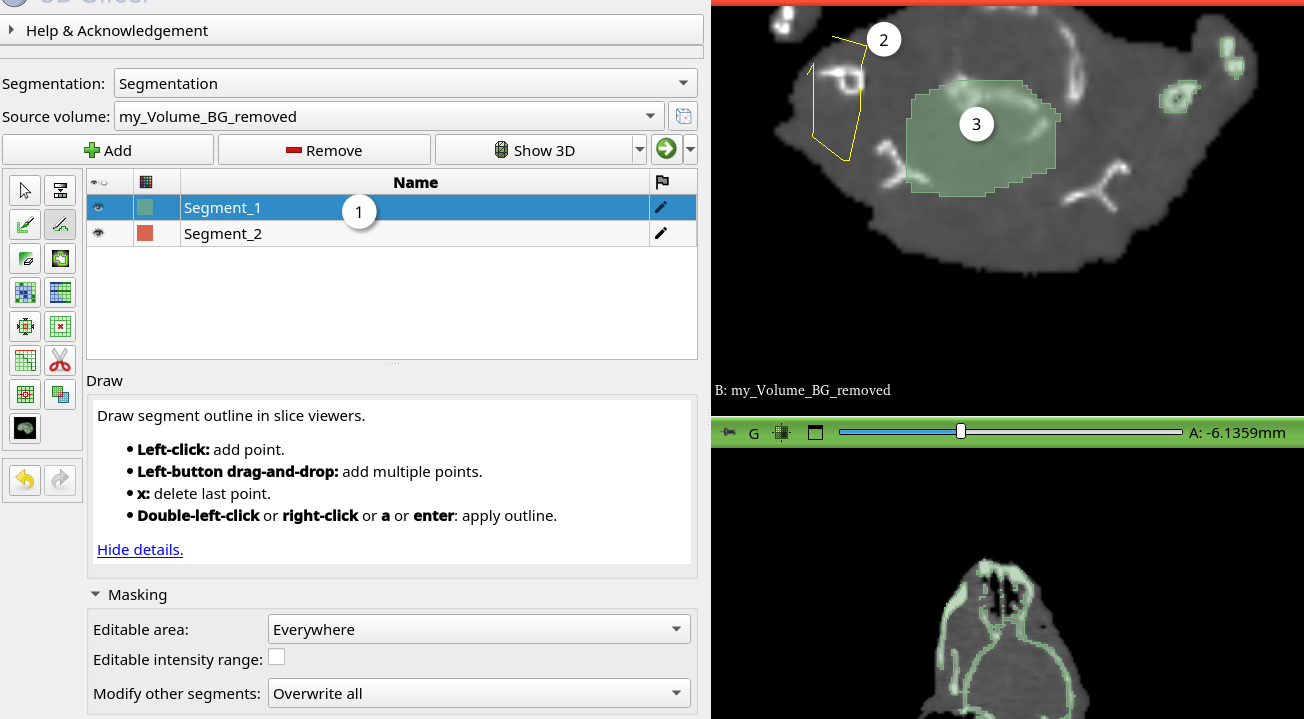
\includegraphics[
			% scale=0.2
			width=1.1\textwidth
		]{draw.png}}
	\caption{Draw tool}\label{fig:draw}
\end{figure}
\noindent
Simple drawing tool.
Make sure the correct segment is selected (\cref{fig:draw}:1).
Click on a 2D view to create points, double click to connect the last point with the first point.
The encompassed area will be filled in (\cref{fig:draw}:3).

\pagebreak
\subsubsection{Level tracing}
\begin{figure}[h]
	\begin{subfigure}{0.2\textwidth}
		\includesvg[
			inkscapelatex=false,
			width = 0.3\textwidth
		]{2d.svg}
	\end{subfigure}
\end{figure}

\begin{figure}[h!]
	\centerline{
		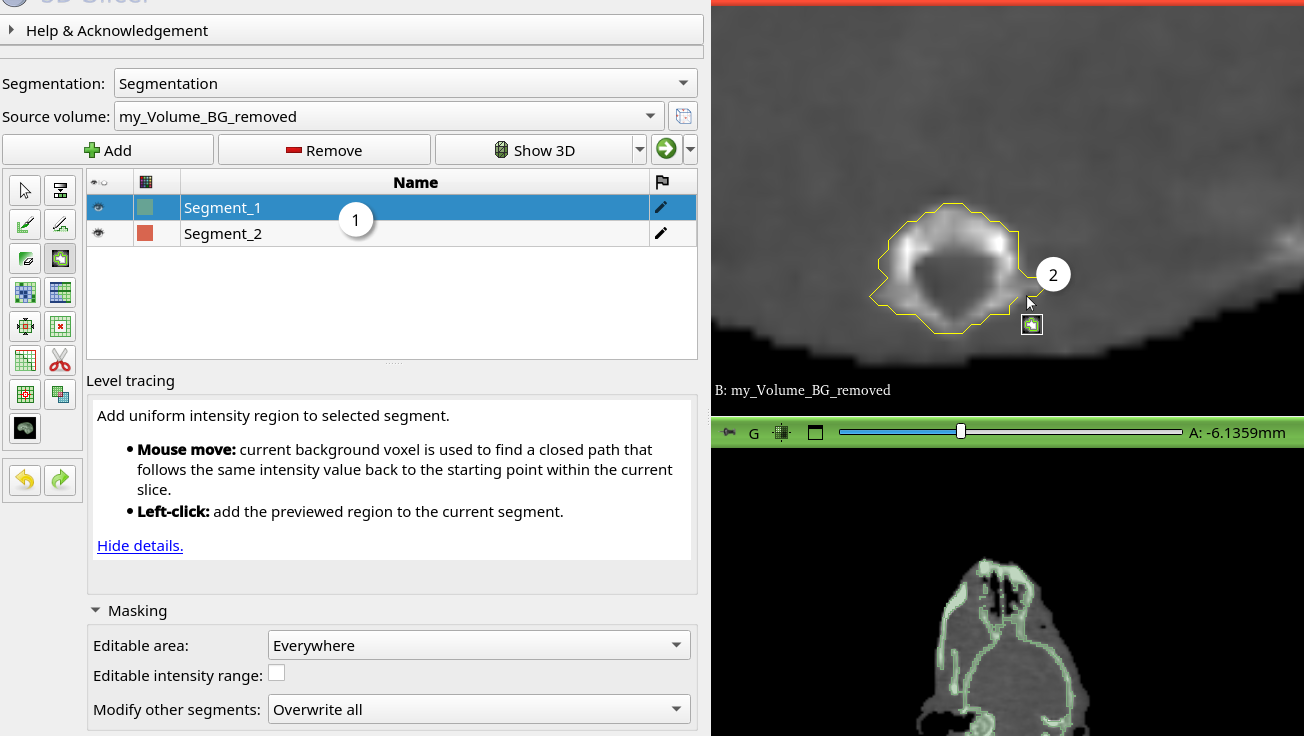
\includegraphics[
			% scale=0.2
			width=1.1\textwidth
		]{levelTracing.png}}
	\caption{Level tracing tool}\label{fig:lT}
\end{figure}
\noindent
\texttt{Level tracing} has a similar role as the \texttt{Draw} tool (\cref{section:draw}).
But instead of manually defining points and connecting them, the tool automatically tries to find areas of similar intensities.
Hover your mouse over a 2D view to see the outline of an area, click to confirm (\cref{fig:draw}:2).

\pagebreak
\subsubsection{Fill between slices}
\begin{figure}[h]
	\begin{subfigure}{0.2\textwidth}
		\includesvg[
			inkscapelatex=false,
			width = 0.3\textwidth
		]{2d.svg}
	\end{subfigure}
	\begin{subfigure}{0.2\textwidth}
		\includesvg[
			inkscapelatex=false,
			width = 0.3\textwidth
		]{performance.svg}
	\end{subfigure}
\end{figure}

\begin{figure}[h!]
	\centerline{
		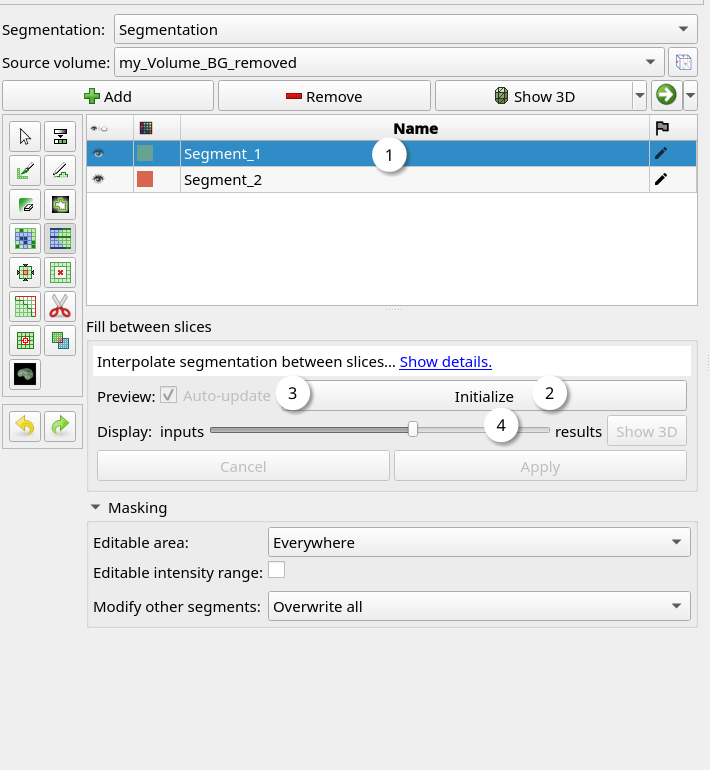
\includegraphics[
			% scale=0.2
			width=1.1\textwidth
		]{fillSlices.png}}
	\caption{Fill between slices tool}\label{fig:fS}
\end{figure}
\noindent
\texttt{Fill between slices} is used similar to \texttt{Grow from seeds} (\cref{section:gfs}).
Start by creating at least one segment and segment a slice with a manual tool.
Skip at least one slice and segment the next slice.
Repeat the last 2 steps until you have covered the desired segmentation volume.
Click on \texttt{Initialize} (\cref{fig:fS}:2) and wait for the interpolation preview to appear in the 2D view area.
The first segmentation will most likely not satisfactory.
Deactivate \texttt{Auto-update} (\cref{fig:fS}:3), switch to the \texttt{Paint} tool and manually paint over the slices with inaccuracies.
Switch back to the \texttt{Fill between slices} tool and click \texttt{Update}.
Repeat until the segmentation is satisfactory.

\pagebreak
\subsubsection{Hollow}
\begin{figure}[h]
	\begin{subfigure}{0.2\textwidth}
		\includesvg[
			inkscapelatex=false,
			width = 0.3\textwidth
		]{2d.svg}
	\end{subfigure}
\end{figure}

\begin{figure}[h!]
	\centerline{
		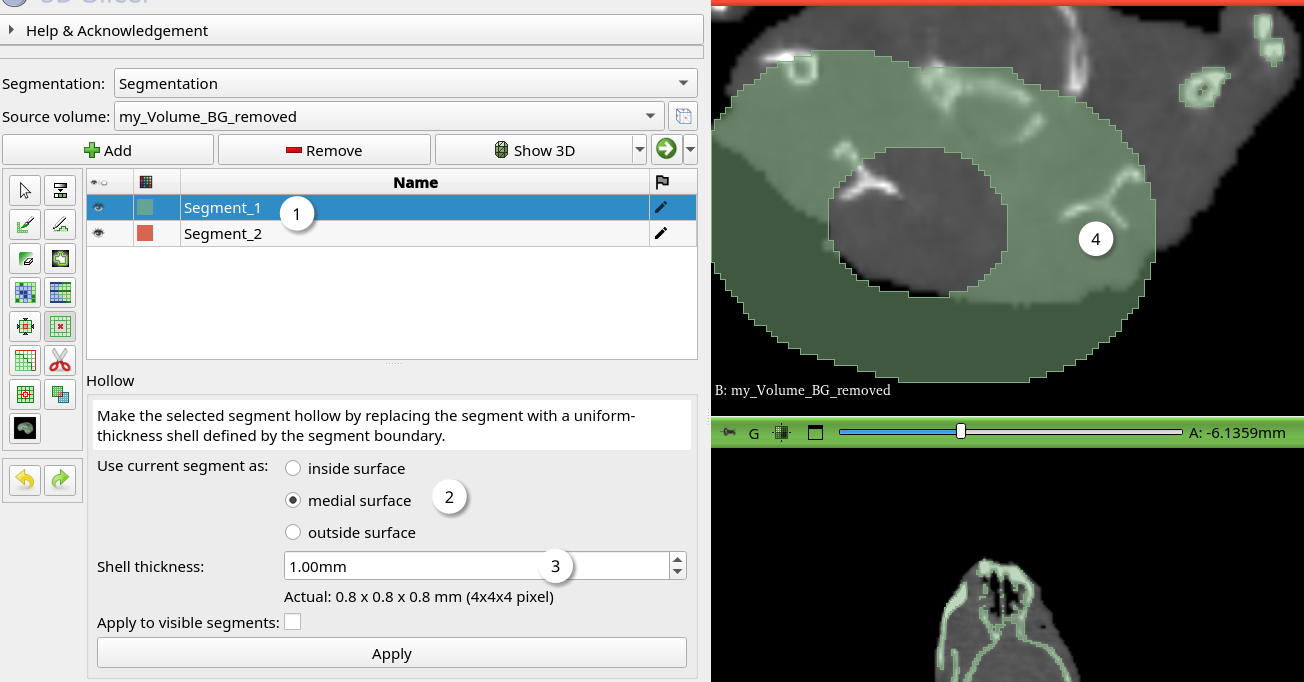
\includegraphics[
			% scale=0.2
			width=1.1\textwidth
		]{hollow.png}}
	\caption{Hollow tool}\label{fig:hollow}
\end{figure}
\noindent
Hollows out a segment (\cref{fig:hollow}:4) by replacing it with a border of a specified thickness (\cref{fig:hollow}:3).
To use this tool, select the desired segment (\cref{fig:hollow}:1), select if the segment should represent the \texttt{inside}, \texttt{medial} or \texttt{outside} border.
Finally set the border thickness (\cref{fig:hollow}:3) and click apply.

\pagebreak
\subsubsection{Scissors}\label{section:scissors}
\begin{figure}[h]
	\begin{subfigure}{0.2\textwidth}
		\includesvg[
			inkscapelatex=false,
			width = 0.3\textwidth
		]{2d.svg}
	\end{subfigure}
	\begin{subfigure}{0.2\textwidth}
		\includesvg[
			inkscapelatex=false,
			width = 0.3\textwidth
		]{3d.svg}
	\end{subfigure}
\end{figure}



\begin{figure}[h!]
	\centerline{
		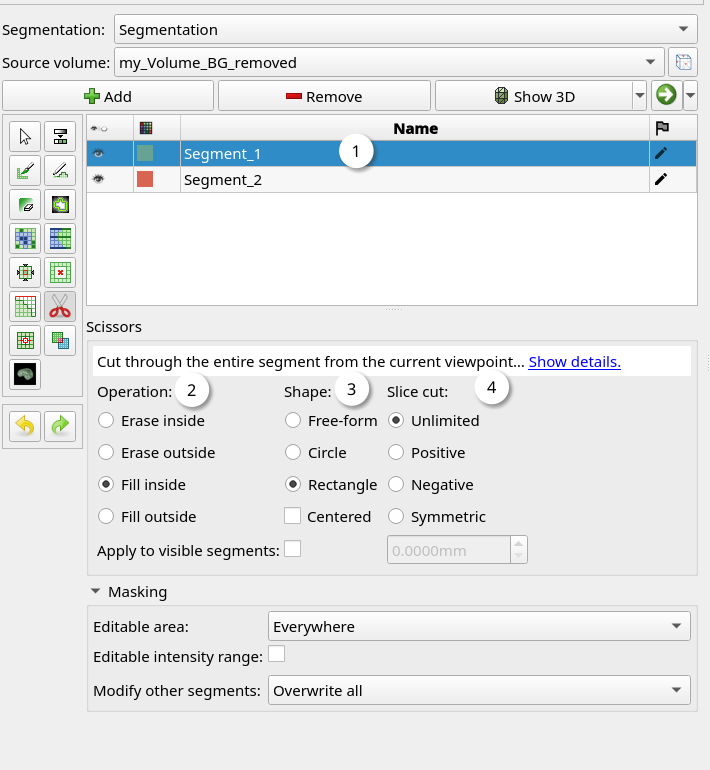
\includegraphics[
			% scale=0.2
			width=1.1\textwidth
		]{scissors.png}}
	\caption{Scissors tool}\label{fig:scissors}
\end{figure}
\noindent
\texttt{Scissors} can be used to cut or fill through a segment.
Select a segment to cut (\cref{fig:scissors}:1) and pick a mode of operation (\cref{fig:scissors}:2).
\begin{description}
	\item [Erase inside] erases already segmented area inside ROI
	\item [Erase outside] erases already segmented area outside ROI
	\item [Fill inside] fills ROI with segment label
	\item [Fill outside] fills everything but the ROI with segment label
\end{description}
Pick a ROI shape (\cref{fig:scissors}:3). \texttt{Centered} means that the ROI will not be drawn from its edge but the center, this may be useful for drawing circular ROIs.
Finally, choose which slices should be affected by the \texttt{Scissors} tool (\cref{fig:scissors}:4).
\begin{description}
	\item [Unlimited] affect all slices
	\item [Positive] only affect slices with a higher slice number than the current one
	\item [Negative] only affect slices with a lower slice number than the current one
	\item [Symmetric] affect both higher and lower slices numbers but only a specific distance
\end{description}

%\pagebreak

\subsubsection{Logical operators}
\begin{figure}[h!]
	\centerline{
		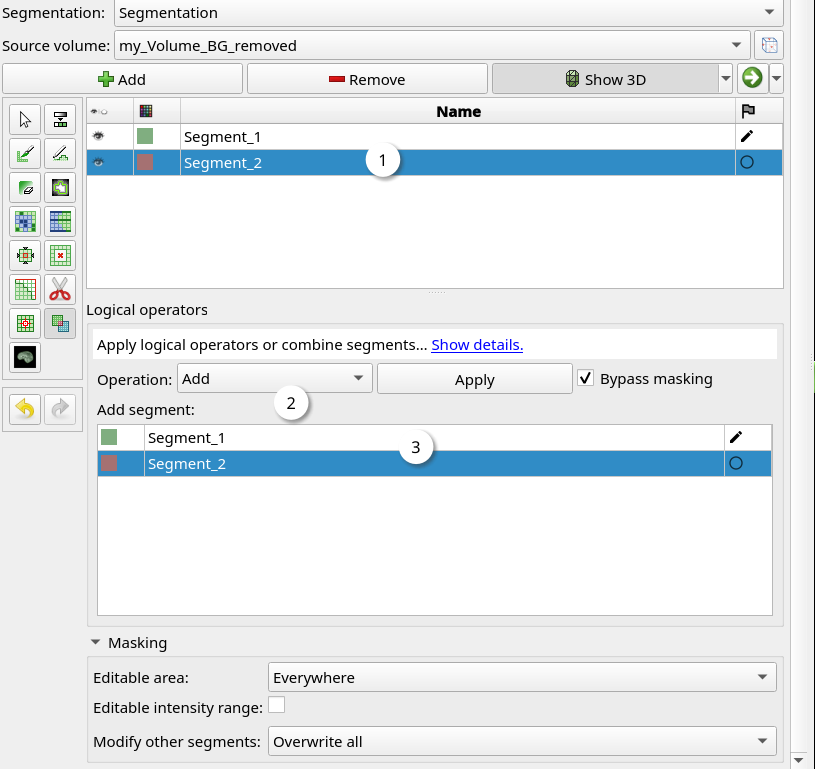
\includegraphics[
			% scale=0.2
			width=1.1\textwidth
		]{bool.png}}
	\caption{Logical operators tool}\label{fig:bool}
\end{figure}
\noindent
Boolean operators processing up to two segments at a time.
First, make sure the correct segment is selected (\cref{fig:bool}:1).
Second, pick an operation (\cref{fig:bool}:2).
\begin{description}
	\item [Copy] copy the segmentation of the modifier segment to the active segment, effectively replacing its segmentation
	\item [Add] combine active and modifier segment
	\item [Subtract] remove overlapping parts of the modifier segment from the active segment
	\item [Intersect] only keep overlapping parts of the modifier segment and the active segment
	\item [Invert] invert the active segment
	\item [Clear] clear the active segment, the same can be achieved via the right click menu and selecting \texttt{Clear selected segments}
	\item [Fill] fill the whole volume with the active segment
\end{description}
Finally, if applicable, pick the modifier segment (\cref{fig:bool}:3) and click apply.

\subsubsection{Undo and Redo}
Undo and Redo work the same as just about in any other software.
The only caveats are that 3D slicer allows only 9 undo operations and that some operations cannot be undone (\cref{section:mask})
\pagebreak

\subsection{Additional segmentation tools}
Some tools are not included with the download of 3D Slicer.
There can be several reasons for this.
Some may not be considered stable enough yet.
Some may have considerable overlap in their use case with a built-in tool.
And some may just not fit 3D Slicer's development direction.
Fortunately, 3D Slicer provides an API which enables the development of extensions.
One such extension is \textquote{SlicerSegmentEditorExtraEffects}\cite{lassoSlicerSegmentEditorExtraEffects2024} by Andras Lasso.
This extension expands the tool section in the \texttt{Segmentation Editor} module with the following tools:
\begin{figure}[h]
	\begin{minipage}{0.4\textwidth}
		\centering
		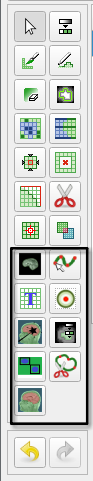
\includegraphics[scale=0.6]{segEE.png}
		\caption{SlicerSegmentEditorExtraEffects}\label{segEE}
	\end{minipage}%
	%
	\begin{minipage}{0.5\textwidth}
		\begin{enumerate} % https://github.com/lassoan/SlicerSegmentEditorExtraEffects
			\item \texttt{Draw Tube}
			\item \texttt{Engrave}
			\item \texttt{Fast Marching}
			\item \texttt{Flood Filling}
			\item \texttt{Split Volume}
			\item \texttt{Surface Cut}
			\item \texttt{Watershed}
			\item \texttt{Local Threshold}
		\end{enumerate}
	\end{minipage}
\end{figure}
\mbox{}

\noindent
Install the extension by clicking on the \texttt{Extensions Manger} in the toolbar (\cref{fig:toolbar}:10).
In the newly opened window, click on \texttt{Install Extensions}, then use the search bar to find ``SegmentEditorExtraEffects''.
Click install and wait for 3D Slicer to ask you for a restart.
The extra tools will be available after restarting 3D Slicer.

\pagebreak
\subsubsection{Draw tube}\label{section:dt}
\begin{figure}[h]
	\begin{subfigure}{0.2\textwidth}
		\includesvg[
			inkscapelatex=false,
			width = 0.3\textwidth
		]{2d.svg}
	\end{subfigure}
	\begin{subfigure}{0.2\textwidth}
		\includesvg[
			inkscapelatex=false,
			width = 0.3\textwidth
		]{3d.svg}
	\end{subfigure}
	\begin{subfigure}{0.2\textwidth}
		\includesvg[
			inkscapelatex=false,
			width = 0.3\textwidth
		]{plugin.svg}
	\end{subfigure}

\end{figure}

\begin{figure}[h!]
	\centerline{
		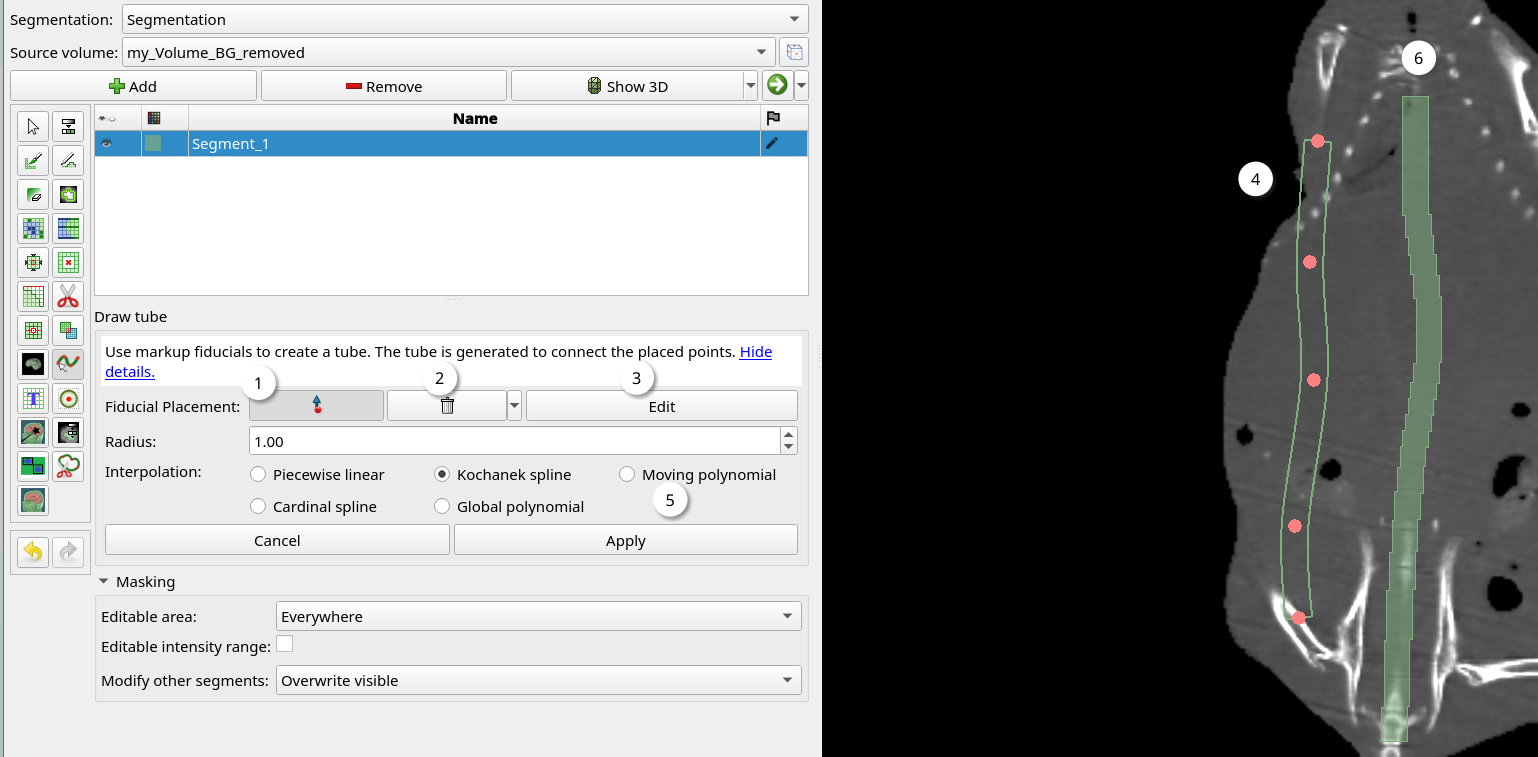
\includegraphics[
			% scale=0.2
			width=1.1\textwidth
		]{drawTube.png}}
	\caption{Draw tube tool}\label{fig:tube}
\end{figure}
\noindent
Draws a tube of fixed radius along a path of points.
First, make sure the desired segment is selected.
Click on \texttt{Place a control point} (\cref{fig:tube}:1) to start drawing.
Create as many control points as you need by clicking on your volume in the 2D or 3D views.
Exit the point creation mode by double left-clicking on the last point or right-clicking anywhere in the view area.
The points can now still be moved freely by clicking and dragging them around.
If you wish to delete the last added point, click on the trashcan icon (\cref{fig:tube}:2).
Pick a tube radius in millimeters and an interpolation algorithm (\cref{fig:tube}:5) by experimenting with the available options and reviewing changes in the preview (\cref{fig:tube}:4).
Click \texttt{Apply} to confirm your changes (\cref{fig:tube}:6).
The result however can still be changed by clicking \texttt{Edit} (\cref{fig:tube}:3).

\pagebreak
\subsubsection{Engrave}
\begin{figure}[h]
	\begin{subfigure}{0.2\textwidth}
		\includesvg[
			inkscapelatex=false,
			width = 0.3\textwidth
		]{2d.svg}
	\end{subfigure}
	\begin{subfigure}{0.2\textwidth}
		\includesvg[
			inkscapelatex=false,
			width = 0.3\textwidth
		]{3d.svg}
	\end{subfigure}
	\begin{subfigure}{0.2\textwidth}
		\includesvg[
			inkscapelatex=false,
			width = 0.3\textwidth
		]{plugin.svg}
	\end{subfigure}
\end{figure}

\begin{figure}[h!]
	\centerline{
		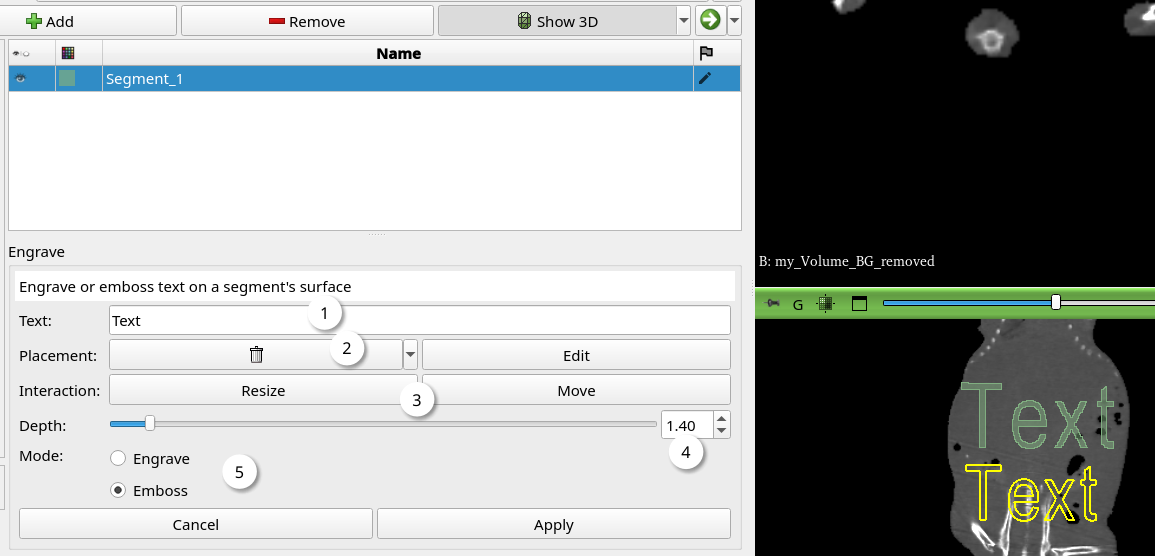
\includegraphics[
			% scale=0.2
			width=1.1\textwidth
		]{engrave.png}}
	\caption{Engrave tool}\label{fig:eng}
\end{figure}
\noindent
Draws or carves out text on a segments surface.
First insert your desired text string (\cref{fig:eng}:1).
Next, click on \texttt{Place a control point} (\cref{fig:eng}:2) and place your text by clicking on the desired position in either the 2D or 3D view area.
Change size and location by selecting either (\cref{fig:eng}:3) and manipulating the text in the view area.
Change the depth of penetration in millimeters by entering a value or dragging the slider (\cref{fig:eng}:4).
Finally choose an operation mode (\cref{fig:eng}:5):
\begin{description}
	\item [Engrave] carve the text out of an existing segment, requires prior segmentation
	\item [Emboss] stamp the text on a segment, requires no prior segmentation
\end{description}

\pagebreak
\subsubsection{Fast Marching}
\begin{figure}[h]
	\begin{subfigure}{0.2\textwidth}
		\includesvg[
			inkscapelatex=false,
			width = 0.3\textwidth
		]{2d.svg}
	\end{subfigure}
	\begin{subfigure}{0.2\textwidth}
		\includesvg[
			inkscapelatex=false,
			width = 0.3\textwidth
		]{plugin.svg}
	\end{subfigure}
\end{figure}
\noindent
Works similar to \texttt{Grow from seeds} (\Cref{section:gfs}) with the big difference that it does not need a ``Background'' segment and can be used on a single segment at a time.
\texttt{Fast Marching} is also considerably faster than \texttt{Grow from seeds}
\texttt{Maximum volume} refers to relative amount of your dataset \texttt{Fast Marching} will try to segment.
Control segmentation leakage via the \texttt{Segment volume} slider.

\subsubsection{Flood Filling}
\begin{figure}[h]
	\begin{subfigure}{0.2\textwidth}
		\includesvg[
			inkscapelatex=false,
			width = 0.3\textwidth
		]{plugin.svg}
	\end{subfigure}
\end{figure}
\noindent
\textquote{Add to the current segment all similar intensity voxels near the clicked position. Generally "Local threshold" effect is recommended instead of this effect because this effect often either cannot prevent leaking into other structures or provides incomplete segmentation.}\cite{lassoSlicerSegmentEditorExtraEffects2024}
This tool has been found to be unreliable and tends to crash often.

\pagebreak
\subsubsection{Split Volume}
\begin{figure}[h]
	\begin{subfigure}{0.2\textwidth}
		\includesvg[
			inkscapelatex=false,
			width = 0.3\textwidth
		]{plugin.svg}
	\end{subfigure}
\end{figure}
\begin{figure}[h!]
	\centerline{
		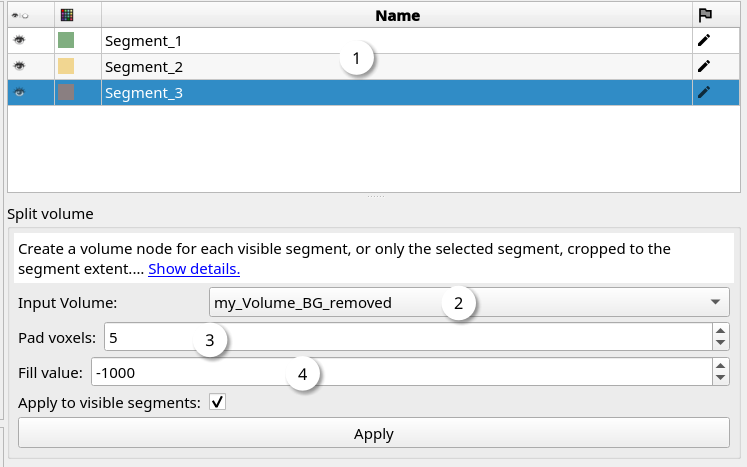
\includegraphics[
			% scale=0.2
			width=1.1\textwidth
		]{split.png}}
	\caption{Split volume tool}\label{fig:split}
\end{figure}
\noindent
Creates a new volume for each segment and requires at least two existing segments.
Start by segmenting parts of your dataset that you wish to split (\cref{fig:split}:1).
Make sure to select the correct input volume (\cref{fig:split}:2).
Set the amount of padding voxels around each segment (\cref{fig:split}:3) and the fill value outside the segmentation (\cref{fig:split}:4).
After clicking \texttt{Apply} the \texttt{Data} module will show some new volumes according to the number of segments you split.

\pagebreak
\subsubsection{Surface Cut}
\begin{figure}[h]
	\begin{subfigure}{0.2\textwidth}
		\includesvg[
			inkscapelatex=false,
			width = 0.3\textwidth
		]{2d.svg}
	\end{subfigure}
	\begin{subfigure}{0.2\textwidth}
		\includesvg[
			inkscapelatex=false,
			width = 0.3\textwidth
		]{3d.svg}
	\end{subfigure}
	\begin{subfigure}{0.2\textwidth}
		\includesvg[
			inkscapelatex=false,
			width = 0.3\textwidth
		]{plugin.svg}
	\end{subfigure}
\end{figure}

\begin{figure}[h!]
	\centerline{
		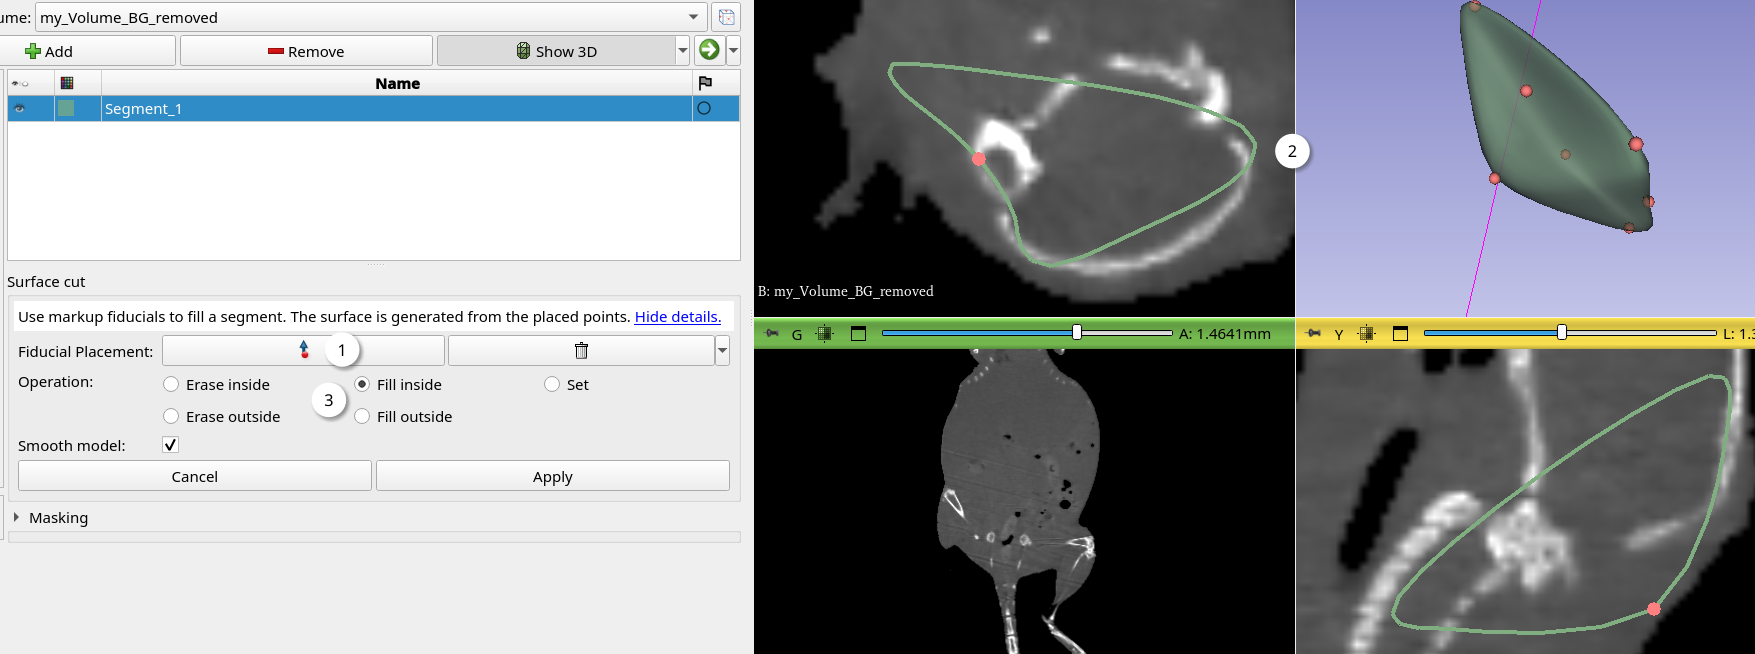
\includegraphics[
			% scale=0.2
			width=1.1\textwidth
		]{surfaceCut.png}}
	\caption{Surface cut tool}\label{fig:sc}
\end{figure}
\noindent
Works similar to \texttt{Draw tube} (\cref{section:dt}) and \texttt{Scissors} (\cref{section:scissors}).
Start by creating fiducial markers (\cref{fig:sc}:1) in the 2D or 3D views (\cref{fig:sc}:2).
Exit fiducial creation mode by either double-clicking on the last fiducial or right-clicking anywhere in the view area.
Modify fidicual placement by clicking and dragging them to the desired position.
Choose an operation mode:
\begin{description}
	\item [Erase inside] erases already segmented area inside fiducial volume
	\item [Erase outside] erases already segmented area outside fiducial volume
	\item [Fill inside] fills fiducial volume with segment label
	\item [Fill outside] fills everything but the fiducial volume with segment label
	\item [Set] fills fiducial volume with segment label
\end{description}

\pagebreak
\subsubsection{Watershed}
\begin{figure}[h]
	\begin{subfigure}{0.2\textwidth}
		\includesvg[
			inkscapelatex=false,
			width = 0.3\textwidth
		]{2d.svg}
	\end{subfigure}
	\begin{subfigure}{0.2\textwidth}
		\includesvg[
			inkscapelatex=false,
			width = 0.3\textwidth
		]{plugin.svg}
	\end{subfigure}
\end{figure}

Works almost identical to \texttt{Grow from seeds}, with the exception that segmentation smoothing factor can be customized via the \texttt{Object scale} setting.
For usage see: \Cref{section:gfs}.

%\pagebreak
\subsubsection{Local Threshold}
\begin{figure}[h]
	\begin{subfigure}{0.2\textwidth}
		\includesvg[
			inkscapelatex=false,
			width = 0.3\textwidth
		]{2d.svg}
	\end{subfigure}
	\begin{subfigure}{0.2\textwidth}
		\includesvg[
			inkscapelatex=false,
			width = 0.3\textwidth
		]{plugin.svg}
	\end{subfigure}
\end{figure}

\begin{figure}[h!]
	\centerline{
		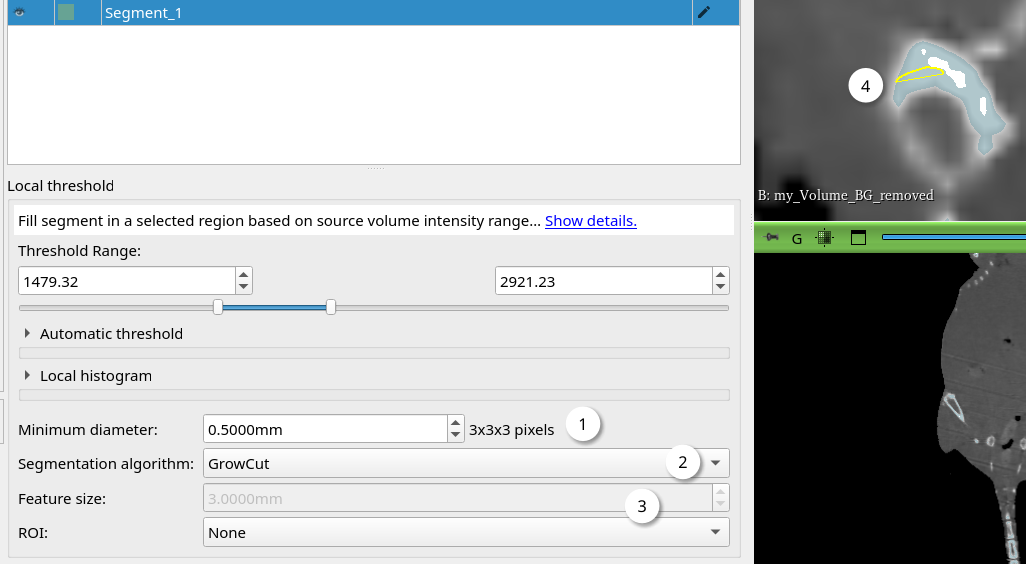
\includegraphics[
			% scale=0.2
			width=1.1\textwidth
		]{locThreshold.png}}
	\caption{Local threshold tool}\label{fig:lt}
\end{figure}
\noindent
ROI based threshold tool.
Start by drawing a ROI in the 2D view area (\cref{fig:lt}:4).
The segmentation algorithm (\cref{fig:lt}:2) will automatically set the lower and upper threshold limit.
If the segmentation is leaky, reduce the \texttt{Minimum diameter}.
This will prevent the segmentation algorithm from considering bridged areas with bridges smaller than the specified amount.
If the watershed algorithm is selected (\cref{fig:lt}:2), \texttt{Feature size} can be used to control the amount of smoothing the algorithm performs.
If you wish to locally restrict the threshold, create and draw a ROI (\cref{fig:lt}:3) before using the tool.

\pagebreak
\section{Performing segmentations}\label{section:quickstart}
Segmenting is now a matter of applying a selection of the tools mentioned above in a meaningful order.
This guide will focus on bone segmentation as this was the authors use case, but the general workflow should apply to most anatomical structures.
\noindent
The next two sections will show you possible workflows.
If you already face performance issues when loading the dataset, start by following the instructions in \cref{section:perf}.

\subsection{Manual}
\begin{description}
	\item [1. Identify the target structure] Navigate to your target structure using the 2D views or visualize it in the \texttt{Volume Rendering} module.
	\item [2. Isolate the target structure] Crop out as much unneeded volume as possible using the method described in \cref{section:crop}. This will not only improve performance, it will also make navigation easier.
	\item [3. Generate a mask for the structure] Using the threshold tool (\cref{section:threshold}) generate a mask for your target structure, in case of this guide bone structures. This will make it almost impossible to accidentally segment unwanted tissue.
	\item [4. (Optional) close holes and smooth edges] If the threshold tool left some holes throughout your target structure it is possible to fix this using a \texttt{Closing} operation (\cref{section:margin}).
	\item [5. Cut away unwanted parts] Use the \texttt{Scissors} tool (\cref{section:scissors}) in 2D or 3D view to cut away unwanted structures from the mask segment.
	\item [6. Create segments] Create a segment for each structure that is going to be segmented and name them accordingly (\cref{fig:manualSeg}:1).
	\item [7. Manually separate structures] Use manual tools like \texttt{Draw, Paint, Draw tube} to separate elements. Overwriting the mask segment created in the third step. This can be achieved by selecting the mask segment as the \texttt{Editable area} in the \texttt{Masking} options (\cref{fig:tM}:6, \cref{fig:manualSeg}:3). Make sure to separate your target structure carefully in all planar views (\cref{fig:manualSeg}:4).
	\item [8. Connect remaining islands] Use the \texttt{Islands} tool (\cref{fig:manualSeg}:2) to connect the middle segment of the last step, effectively finishing the segmentation.\end{description}
\begin{figure}[h!]
	\centerline{
		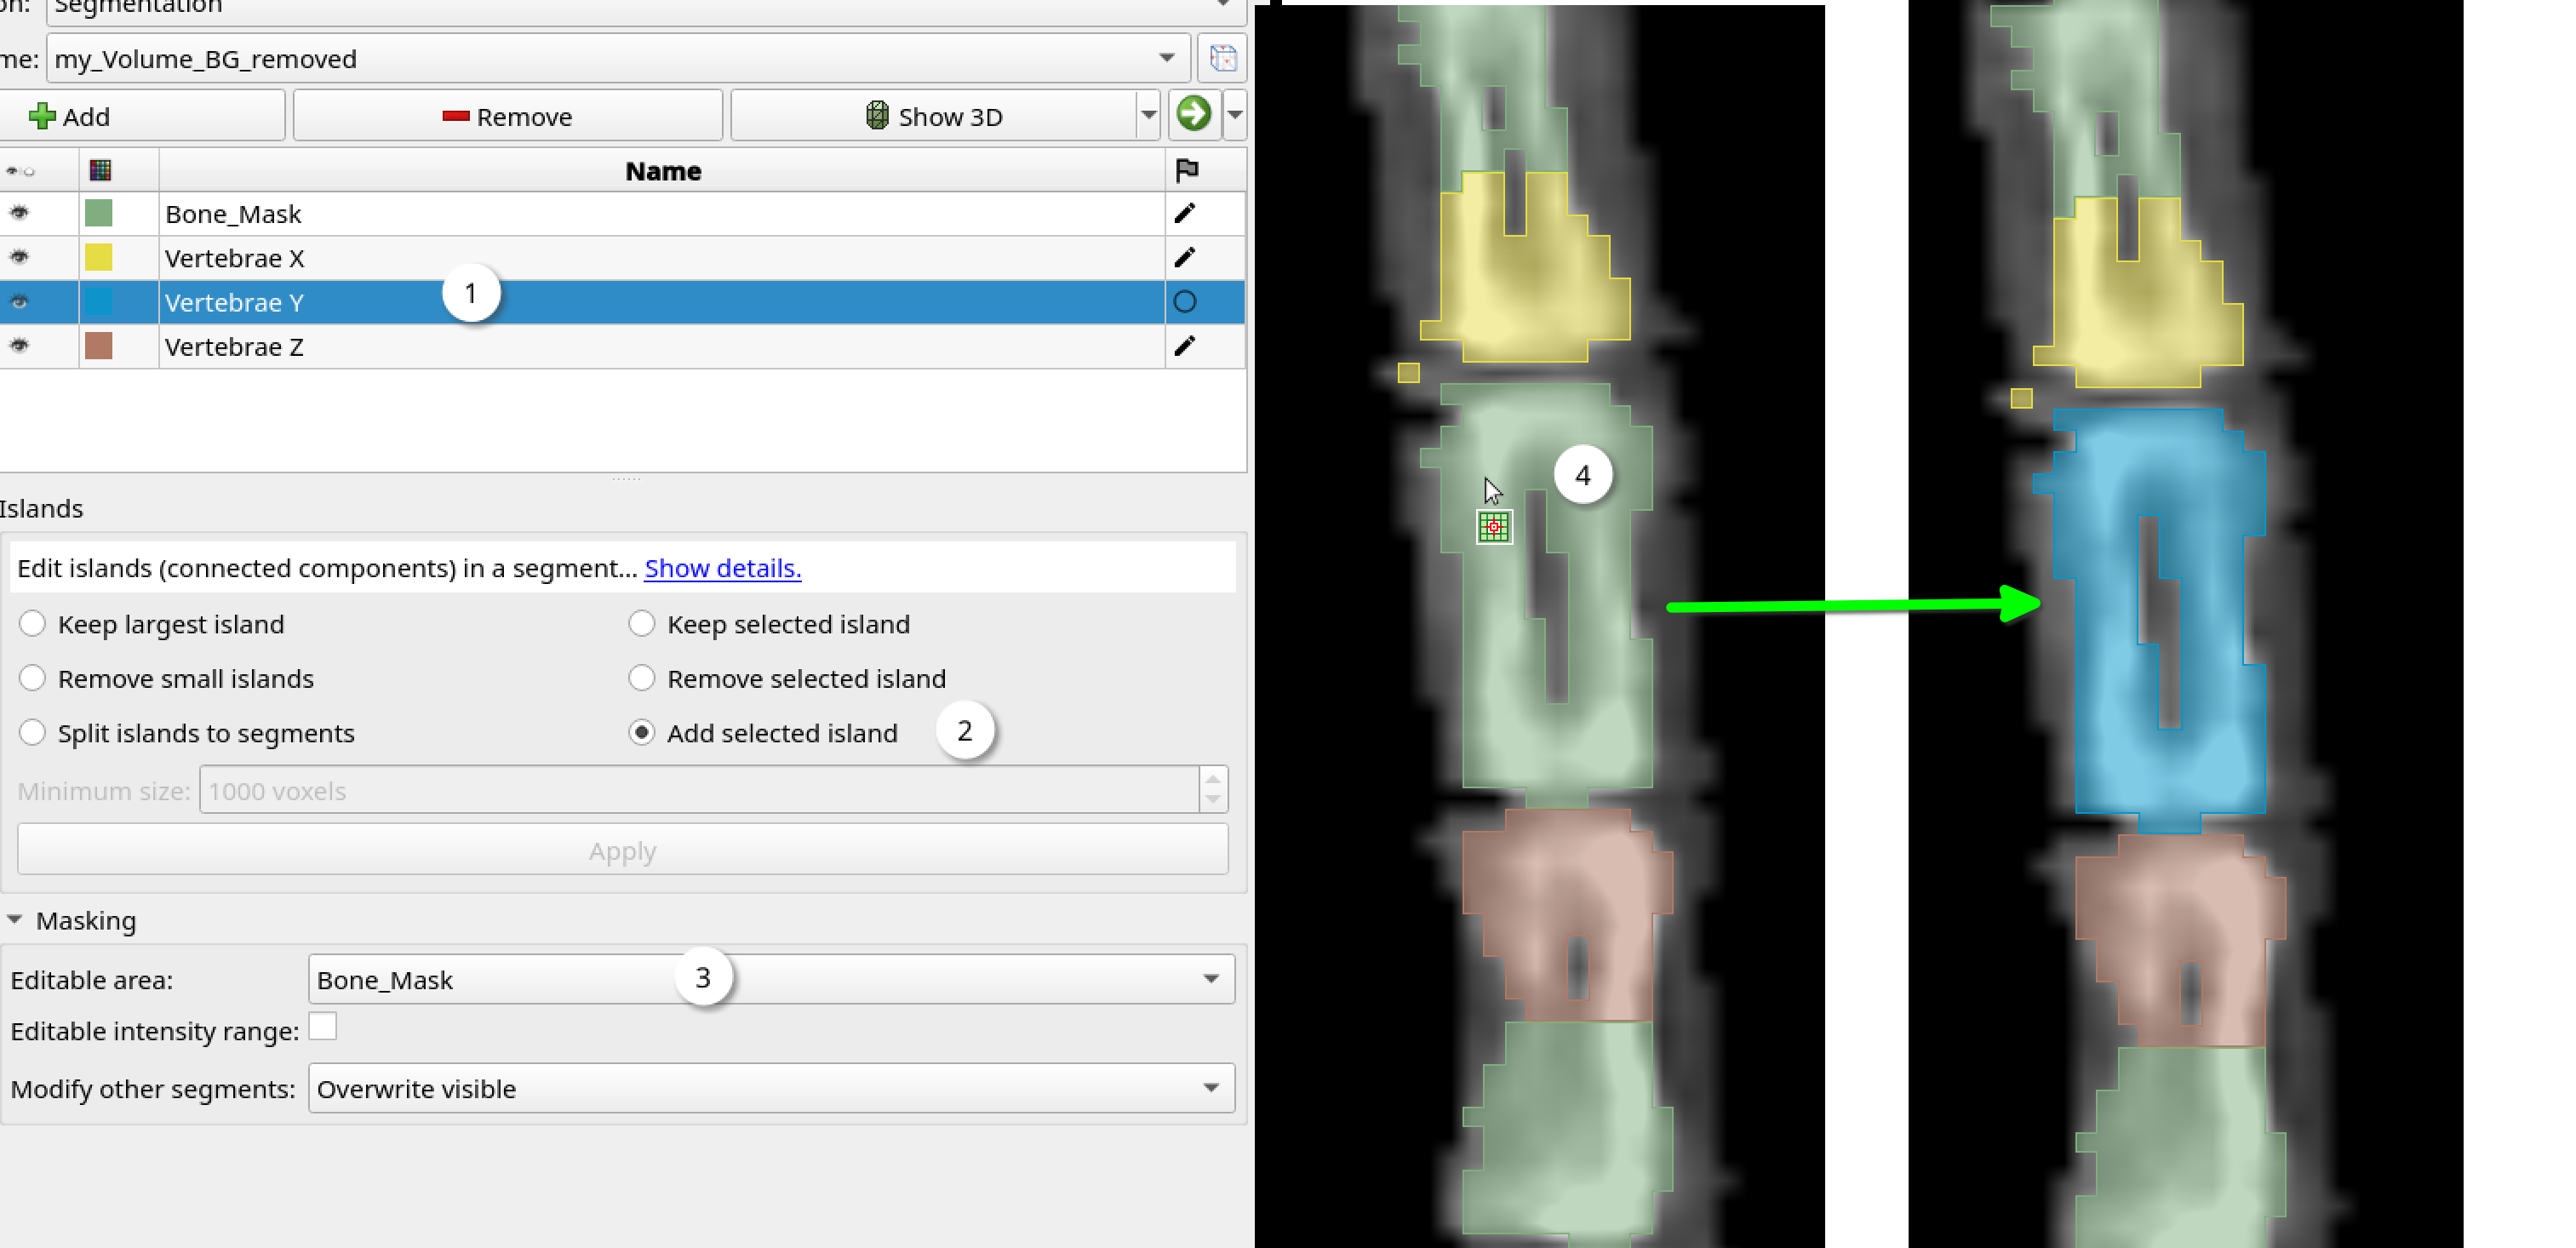
\includegraphics[
			% scale=0.2
			width=1.1\textwidth
		]{manualSeg.png}}
	\caption{Manual segmentation via islands}\label{fig:manualSeg}
\end{figure}

\pagebreak
\subsection{Semi-Automatic}
\begin{description}
	\item [1. Identify the target structure] Navigate to your target structure using the 2D views or visualize it in the \texttt{Volume Rendering} module.
	\item [2. Isolate your target structure] Crop out as much unneeded volume as possible using the method described in \cref{section:crop}. This will not only improve performance, it will also make navigation easier.
	\item [3. Determine threshold for masking] Using the threshold tool (\cref{section:threshold}) generate a mask for your target structure, in case of this guide bone structures. Alternatively just use the threshold tool to determine the upper and lower limits and use them in the masking tab of the chosen semi-automatic segmentation tool.
	\item [4. Create segments] Create a segment for each structure that is going to be segmented and name them accordingly. If you plan to use \texttt{Grow from seeds} (\cref{section:gfs}) also create a background label.
	\item [5. Paint seeds] Manually paint seeds inside the structures you wish to segment. Make the seeds evenly spread throughout the structure and add extra seeds where structures border. When using \texttt{Grow from seeds} also do this for the background segment.
	\item [6. Perform semi-automatic segmentation] Let the tool calculate a segmentation based on your seeds. Improve the segmentation by going back to step 5 and adding more seeds. Repeat until the result is sufficiently accurate.
\end{description}

\pagebreak
